\documentclass[semifinal]{cpecmu}
\usepackage{multirow}
\usepackage{pgfplots}
\usepackage{pgf-pie}
%% This is a sample document demonstrating how to use the CPECMU
%% project template. If you are having trouble, see "cpecmu.pdf" for
%% documentation.

\projectNo{S001-2}
\acadyear{2020}

\titleTH{หนีจากวังวน}
\titleEN{Escape}

\author{กรวิชญ์ บัวคำปัน}{Goravit Buakampun}{610610567}
\author{กิตติพงษ์ ไมล์หรือ}{Kittipong Milerue}{610610570}

\cpeadvisor{chinawat}
\cpecommittee{narathip}
\cpecommittee{arnan}

%% Some possible packages to include:
\usepackage[final]{graphicx} % for including graphics

%% Add bookmarks and hyperlinks in the document.
\usepackage[colorlinks=true,allcolors=Blue4,citecolor=red,linktoc=all]{hyperref}

%% Set up commenting
\iffinal
  \usepackage[disabled]{authcomments}
\else
  \usepackage{authcomments}
\fi
\newcommenter{CI}{0.0,0.5625,0.0}  % green
\newcommenter{GB}{0.0,0.5625,0.0}

%% Needed just by this example, but maybe not by most reports
\usepackage{afterpage} % for outputting
\usepackage{pdflscape} % for landscape figures and tables. 

\usepackage{amsmath}
%% Some other useful packages. Look these up to find out how to use
%% them.
% \usepackage{natbib}    % for author-year citation styles
% \usepackage{txfonts}
% \usepackage{appendix}  % for appendices on a per-chapter basis
% \usepackage{xtab}      % for tables that go over multiple pages
% \usepackage{subfigure} % for subfigures within a figure
% \usepackage{pstricks,pdftricks} % for access to special PostScript and PDF commands
% \usepackage{nomencl}   % if you have a list of abbreviations

%% if you're having problems with overfull boxes, you may need to increase
%% the tolerance to 9999
% \tolerance=9999

\bibliographystyle{plain}
% \bibliographystyle{IEEEbib}

% \renewcommand{\topfraction}{0.85}
% \renewcommand{\textfraction}{0.1}
% \renewcommand{\floatpagefraction}{0.75}

%% Example for glossary entry
%% Need to use glossary option
%% See glossaries package forcomplete documentation.
\ifglossary
  \newglossaryentry{lorem ipsum}{
    name=lorem ipsum,
    description={derived from Latin dolorem ipsum, translated as ``pain itself''}
  }
\fi

%% Uncomment this command to preview only specified LaTeX file(s)
%% imported with \include command below.
%% Any other file imported via \include but not specified here will not
%% be previewed.
%% Useful if your report is large, as you might not want to build
%% the entire file when editing a certain part of your report.
% \includeonly{chapters/intro,chapters/background}

\begin{document}
\maketitle
\makesignature

\ifproject
\begin{abstractTH}

$\>$วิทยาการคำนวณ (computing science) เป็นวิชาที่จะเข้ามาแทนวิชาคอมพิวเตอร์หรือ วิชาด้านเทคโนโลยีในที่สอนอยู่ในปัจจุบัน 
รายละเอียดของวิชาวิทยาการคำนวณ ไม่ใช่แค่ให้ผู้เรียน เรียนแค่การเขียนโปรแกรมคอมพิวเตอร์ หรือ เรียนรู้เกี่ยวกับการใช้คอมพิวเตอร์แค่ขั้นพื้นฐานเท่านั้น 
แต่วิชานี้ยังสอนให้เด็ก ๆ มีกระบวนการคิดเชิงวิเคราะห์อย่างเป็นระบบและสามารถนำมาปรับใช้เพื่อแก้ไขปัญหาได้อย่างสร้างสรรค์ 
ซึ่งในรายวิชานี้ได้มีการกำหนดขอบเขตการเรียนการสอนเอาไว้ 3 องค์ความรู้ ได้แก่ 1.การคิดเชิงคำนวณ 
(computational thinking) 2.พื้นฐานความรู้ด้านเทคโนโลยีดิจิทัล (digital technology) 
3.พื้นฐานการรู้เท่าทันสื่อและข่าวสาร (media and information literacy) 
โดยปัญหาที่ทางผู้พัฒนาได้ไปสำรวจมาในโรงเรียนพื้นที่รอบนอกชั้นประถมศึกษา คือ ทางโรงเรียนไม่มีศักยภาพพอที่จะสอนวิชาวิทยาการคำนวณ 
เพราะบุคลากรไม่พร้อม จบไม่ตรงสาย ทำให้เด็กนักเรียนไม่ได้เรียนวิชาวิทยาการคำนวณอย่างที่ควรเป็นในหลักสูตรของกระทรวงศึกษาธิการ 
ซึ่งทางผู้พัฒนาได้เล็งเห็นว่า การที่จะนำเสนอรูปแบบการเรียนการสอนในรูปแบบที่เด็กสามารถเรียนรู้ได้ด้วยตัวเอง และสนุกไปกับมัน 
เลยทำให้เกิดโครงการ เกมเสริมทักษะวิทยาการคำนวณ ขึ้นมา

$\>$โครงการ หนีออกจากวังวน (Escape) จะเน้นด้านการคิดเชิงคำนวณ 
สามารถช่วยแก้ไขปัญหาการที่นักเรียนไม่ได้เรียนวิชาวิทยาการคำนวณอย่างที่ควรเป็น 
โดยทางผู้พัฒนาจะนำ block code เข้ามาใช้ในตัวเกมเพื่ออิงตามหลักสูตรวิชาวิทยาการคำนวณของกระทรวงศึกษาธิการ 
ที่ได้มีการเรียนการสอนโดยใช้ scratch ที่เป็น block code เหมือนกัน 
โดยตัวเกมจะเป็นการที่ผู้เล่น (นักเรียน) นำ block code มาวางวางเพื่อบังคับตัวละครในเกมเพื่อแก้ไขปัญหาในแต่ละด่านที่ได้ออกแบบอิงตามแบบฝึกหัดหนังสือของ 
สสวท. วิชาวิทยาการคำนวณ
% \enskip ภาควิชาวิศวกรรมคอมพิวเตอร์จึงได้จัดทำต้นแบบรูปเล่มรายงานโดยใช้ระบบจัดเตรียมเอกสาร
% \LaTeX{} เพื่อช่วยให้นักศึกษาเขียนรายงานได้อย่างสะดวกและรวดเร็วมากยิ่งขึ้น
\end{abstractTH}

\begin{abstract}
    
$\>$Computing science is a subject that will replace Computer or Technology subjects currently being taught
details of computational science Not just for students Learn only computer programming or learn only the basics of using computers.
But this course also teaches children to have a systematic analytical thinking process and be able to apply it to creative problem solving.
which in this course has set the scope of teaching out 3 body of knowledge: 1. Computational thinking
2. Fundamentals of digital technology knowledge 3. Fundamentals of media and information literacy
The problem that the developers have explored in schools in the outer areas of primary school is that the school does not have enough potential to teach computational science.
Because the personnel are not ready, the graduates are not in line, causing the students to not study computational science as they should in the curriculum of the Ministry of Education.
which the developer has foreseen To present a teaching style in a way that children can learn on their own. and enjoy it
thus causing the project A game to enhance math skills

$\>$The Escape project focuses on computational thinking.
It can help solve the problem of students not taking computational science courses as they should be.
The developer will use the block code in the game based on the Ministry of Education's computational science curriculum.
that has been taught using scratch that is the same block code
In the game, players (students) place block codes to control the characters in the game to solve problems in each level designed based on the book exercises of
NSTDA in Computational Science

Make sure your abstract sits inside the \texttt{abstract} environment.
\end{abstract}

\iffalse
\begin{dedication}
This document is dedicated to all Chiang Mai University students.

Dedication page is optional.
\end{dedication}
\fi % \iffalse

\begin{acknowledgments}
โครงการ หนีออกจากวังวน (Escape) 
นี้จะประสบความสำเร็จไม่ได้หากไม่ได้รับการสนับสนุนจาก 
คณะ วิศวกรรมศาสตร์ มหาวิทยาลัยเชียงใหม่ 
ในด้านการอำนวยความสะดวกและสถานที่ในการพัฒนาโปรแกรม 
อาจารย์ ชินวัตร อิศราดิสัยกุล ที่ให้คำปรึกษาในการพัฒนาโปรแกรม 
ทีมผู้ร่วมพัฒนาที่คอยช่วยเหลือกันในการพัฒนาโปรแกรม 
นากจากนี้ทางคณะผู้พัฒนายังได้รับกำลังใจจากบิดมารดาพี่น้องอาจารย์และ
เพื่อนของผู้พัฒนา อำนวยความสะดวกและให้คำปรึกษาด้านโปรแกรม 
% \texttt{acknowledgment} environment.

\acksign{2020}{5}{25}
\end{acknowledgments}%
\fi % \ifproject

\contentspage

\ifproject
\figurelistpage

\tablelistpage
\fi % \ifproject

% \abbrlist % this page is optional

% \symlist % this page is optional

% \preface % this section is optional


\pagestyle{empty}\cleardoublepage
\normalspacing \setcounter{page}{1} \pagenumbering{arabic} \pagestyle{cpecmu}

\chapter{\ifcpe บทนำ\else Introduction\fi}

\section{\ifcpe ที่มาของโครงงาน\else Project rationale\fi}
ในปี พ.ศ. 2560 กระทรวงศึกษาธิการได้เพิ่มหลักสูตรวิชาวิทยาการคำนวณ~\cite{cpc}มาในรายวิชาวิทยาศาสตร์
 เพื่อให้เด็กนักเรียนได้มีความพร้อมในยุคเทคโนโลยีดิจิทัล 
และเป็นการเสริมความรู้ในด้านทักษะการคิดเชิงคำนวณ 
พื้นฐานด้านเทคโนโลยีดิจิทัล และ พื้นฐานการรู้เท่าทันสื่อและข่าวสาร\par

ผู้พัฒนาได้มีความสนใจในการเข้าไปศึกษาเรียนรู้เกี่ยวกับตัวหลักสูตรในด้านการเรียนการสอน
จากประสบการณ์ของผู้พัฒนาที่ได้คลุกคลีกับโรงเรียนรอบนอก
ทำให้เล็งเห็นถึงการกระจายความรู้ที่เป็นไปได้ยากในโรงเรียนรอบนอก ผู้พัฒนาเลยทำการที่จะสำรวจและจากการลงพื้นที่โรงเรียนรอบนอก
 ได้แก่ โรงเรียนบ้านออนใต้, โรงเรียนมิตรมวลชน และโรงเรียนบ้านดอยเต่า\par

จากผลการสำรวจได้พบเจอกับปัญหาคือ โรงเรียนรอบนอกไม่สามารถได้รับความรู้ในรายวิชาวิทยาการคำนวณได้อย่างมีประสิทธิภาพ 
ไม่ว่าจะเป็นการที่มีบุคลากรครูที่ไม่เพียงพอ หรือบุคลากรครูที่สอนรายวิชาวิทยากรคำนวณนั้นจบไม่ตรงสาย 
ทำให้เกิดความเหลื่อมล้ำทางการศึกษาส่งผลให้เด็กนักเรียนไม่ชอบ หรือไม่รู้จักวิชาวิทยาการคำนวณว่าจริง ๆ 
แล้ววิชานี้คือวิชาอะไร ถึงแม้ว่าทางกระทรวงศึกษาธิการได้มีการผลักดันหลักสูตรรายวิชาวิทยาการคำนวณเป็นอย่างมากแล้วก็ตาม\par

จากอีกหนึ่งผลสำรวจได้ว่าเด็กนักเรียนนั้นชอบเล่นเกมที่เป็นแนว Puzzle แก้ปัญหาเป็นด่านๆ ผู้พัฒนาเลยมีความคิดว่าจะทำสื่อในรูปแบบที่นักเรียนมีความสนใจนั้นก็คือเกม
ซึ่งจะทำให้นักเรียนได้มีปฏิสัมพันธ์กับรายวิชาวิทยาการคำนวณในรูปแบบที่นักเรียนชอบ และการคิดเชิงคำนวณเป็นสิ่งที่เป็นพื้นฐานในการแก้ไขปัญหาต่างๆ ในชีวิตประจำวัน
เลยทำให้เกิดโครงงาน Escape นี้ขึ้นมาเพื่อนำเสนอการเรียนการสอนวิชาวิทยาการคำนวณในรูปแบบของเกม
โดยเราจะเน้นไปที่ การคิดเชิงคำนวณ

\section{\ifcpe วัตถุประสงค์ของโครงงาน\else Objectives\fi}
\begin{enumerate}
    \item เพื่อช่วยแก้ไขปัญหาความเหลื่อมล้ำทางการศึกษาโดยเป็นเครื่องมือในการสอนโดยนำเสนอในรูปแบบของเกม
    \item เพื่อให้นักเรียนสามารถนำความรู้ที่ได้ไปปรับใช้ในรายวิชา และในชีวิตจริง และสามารถผลิตเยาวชนที่มีคุณภาพให้กับประเทศได้
    \item เพื่อเป็นการผลักดัน และแสดงให้เห็นถึงความสำคัญของหลักสูตรวิชาวิทยาการคำนวณ
\end{enumerate}

\section{\ifcpe ขอบเขตของโครงงาน\else Project scope\fi}
% \CIreply{ไม่ชัดเจนว่าจะทำอะไร จะไม่ทำอะไร}
ตัวเกมทำงานได้ในระบบ Android เท่านั้นแต่ว่าอนาคตจะมีการรอบรับระบบอื่น ๆ 
เข้ามาเช่น iOS, PC, Web App เป็นตัน 
และในแต่ละด่านนั้นจะสร้างขึ้นโดยอิงจากหลักสูตรที่อยู่ในหนังสือวิทยาการคำนวณของกระทรวง
โดยจะสามารถสร้างด่านโดยการอ่านไฟล์ text

\subsection{\ifcpe ขอบเขตด้านฮาร์ดแวร์\else Hardware scope\fi}
เป็นเกมที่ต้องเล่นบน smart phone ที่ทำงานบนระบบปฏิบัติการ Android โดยในอนาคตอาจจะมีการการพัฒนาให้สามารถเล่นบน iOs, PC, VR ได้

\subsection{\ifcpe ขอบเขตด้านซอฟต์แวร์\else Software scope\fi}
ตัวเกมต้องใช้ Android version 5.0 'Lollipop' หรือสูงกว่าและ API level 21 หรือสูงกว่า
โดยในอนาคตอาจจะมีการการพัฒนาให้สามารถเล่นบน iOS ได้

\section{\ifcpe ประโยชน์ที่ได้รับ\else Expected outcomes\fi}
ประโยชน์ที่ได้รับที่คาดไว้มีอยู่ 2 ด้าน 
\begin{enumerate}
    \item นักเรียน นักเรียนได้เรียนรู้ในตัววิชาเพื่อนำไปแก้ไขปัญหาในวิชาเรียนรวมไปถึงปัญหาในชีวิตประจำวันได้
    \item โรงเรียน เมื่อนักเรียนสามารถแก้ไขปัญหาต่างๆ ได้ ทางโรงเรียนเองสามารถผลิตเด็กที่มีคุณภาพเพื่อออกไปสู่สังคัมได้ 
\end{enumerate}
% \CIreply{เขียนแยกทีละประเด็น}

\section{\ifcpe เทคโนโลยีและเครื่องมือที่ใช้\else Technology and tools\fi}

\subsection{\ifcpe เทคโนโลยีด้านฮาร์ดแวร์\else Hardware technology\fi}
ไม่มี

\subsection{\ifcpe เทคโนโลยีด้านซอฟต์แวร์\else Software technology\fi}
ตัว Game Engine ใช้ Unity3d~\cite{utb,ud} ตัว Code Block ใช้ Google Blockly~\cite{gb}
ส่วนด้านแสดงผลตัว Block Code ใช้ HTML และ JavaScript โดยใช้ Google Firebase~\cite{fb} ในการ Host

\section{\ifcpe แผนการดำเนินงาน\else Project plan\fi}
\CIreply{revise}
\begin{plan}{11}{2020}{10}{2021}
    \planitem{11}{2020}{11}{2020}{ค้นหาปัญหา และ สืบค้นข้อมูลเพื่อนำมาใช้เป็นหัวข้อของโครงการ}
    \planitem{11}{2020}{12}{2020}{ศึกษาข้อมูลเกี่ยวกับการใช้งานโปรแกรมที่ใช้ในการพัฒนา}
    \planitem{12}{2020}{12}{2020}{เริ่มทดลองระบบและทดลองใช้ Asset ของ Unity}
    \planitem{1}{2021}{1}{2021}{ออกแบบเกมเพลย์ของเกม}
    \planitem{1}{2021}{1}{2021}{ทำการออกแบบแผนที่ภายในเกม}
    \planitem{2}{2021}{2}{2021}{ศึกษาเกี่ยวกับ Blockly เพื่อใช้สำหรับสร้าง และพัฒนา Block Code}
    \planitem{2}{2021}{3}{2021}{ทดสอบการใช้งานและแก้ไข Block Code ที่สร้างขึ้น}
    \planitem{4}{2021}{4}{2021}{เริ่มออกแบบฟังก์ชันภายในเกม}
    \planitem{4}{2021}{5}{2021}{ศึกษาเกี่ยวกับระบบ Hosting ด้วย Firebase ให้สามารถใช้งานกับ Unity ได้}
    \planitem{5}{2021}{5}{2021}{ทดสอบการใช้งานระบบ Hosting ของ Firebase ให้ใช้งานกับ Unity ได้}
    \planitem{6}{2021}{9}{2021}{พัฒนา Block Code และ ทดสอบระบบกับ Firebase และ Unity ให้เสร็จสิ้น}
    \planitem{6}{2021}{9}{2021}{ทำ UX/UI และ องค์ประกอบภายในเกม}
    \planitem{7}{2021}{10}{2021}{ทดสอบเกมโดยรวม ทำการค้นหาบัคและแก้ไขปัญหาที่เกิดขึ้น}


\end{plan}
\CIreply{มีแผนการดำเนินงานแค่นี้จริงหรือ?ลงรายละเอียด}

\section{\ifcpe บทบาทและความรับผิดชอบ\else Roles and responsibilities\fi}
ตัวเกมจะแบ่งเป็นอยู่ 2 ส่วน คือส่วนที่อยู่บนเว็บซึ่งจัดการด้านตัว Block Code และ ฝั่ง Unity จะจัดการด้านแสดงผล โดยแบ่งไปอีก
2 ส่วนย่อย คือ UI , Mechanic โดยบทบาทจะแบ่งเป็น
\begin{enumerate}
    \item กรวิชญ์ บัวคำปัน จัดการด้านเว็ป, เกม Mechanic, และ UI
    \item กิตติพงษ์ ไมล์หรือ จัดการด้าน UI
\end{enumerate}

\section{\ifcpe%
ผลกระทบด้านสังคม สุขภาพ ความปลอดภัย กฎหมาย และวัฒนธรรม
\else%
Impacts of this project on society, health, safety, legal, and cultural issues
\fi}

% แนวทางและโยชน์ในการประยุกต์ใช้งานโครงงานกับงานในด้านอื่นๆ รวมถึงผลกระทบในด้านสังคมและสิ่งแวดล้อมจากการใช้ความรู้ทางวิศวกรรมที่ได้
เกิดเป็นสื่อการเรียบการสอนเพื่อให้เด็กนักเรียนสามารถเข้าถึงตััววิชาวิทยาการคำนวณในรูปแบบที่เด็กชื่นชอบและ จะทำให้เด็กนั้นมีความเข้าใจ
ในรายวิชา เพื่อนำไปใช้ในการแก้ปัญหาในการเรียน หรือแม้กระทั่งปัญหาในชีวิตจริง
\chapter{\ifcpe ทฤษฎีที่เกี่ยวข้อง\else Background Knowledge and Theory\fi}
\label{bg}

\section{Model View Controller (MVC)}
โครงงานนี้ใช้ design pattern MVC~\cite{mvc} ซึ่งแบ่งออกเป็น 3 ส่วนหลักๆ ดังรูปที่ \ref{mvc} ได้แก่ 
\begin{enumerate}
    \item Model
    \item View
    \item Controller
\end{enumerate}

  \begin{figure}[h!]
    \begin{center}
    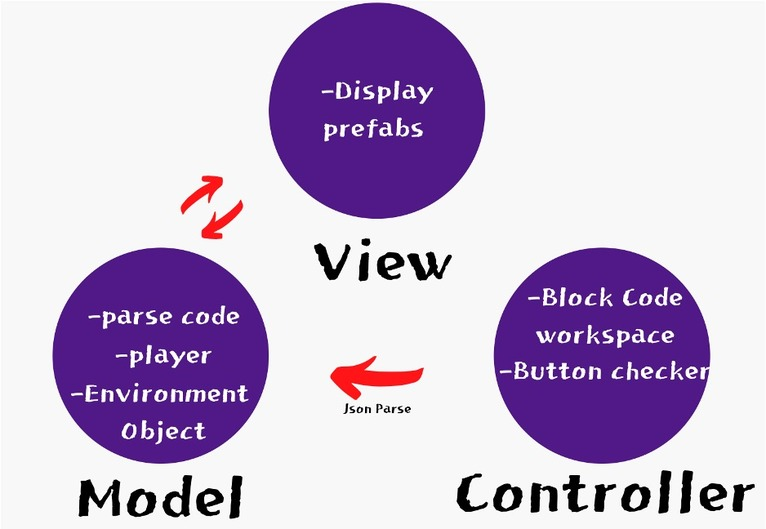
\includegraphics{pic/pic1.jpg}
    \end{center}
    \caption[Design Pattern MVC]{Design Pattern MVC}
    \label{mvc}
    \end{figure}
  

\subsection{Model}
 ในส่วนของ model จะเป็นการจัดการแปลงจาก block code ให้เป็น C\# เพื่อทำให้เกิด events ต่างๆ เช่นการเดิน การหมุน
 และการกระโดด เป็นต้น โดยที่ model จะรับ block code มาจาก controller ในรูปของ JSON
 และจะทำการแปลงเป็น C\# เพื่อสั่งให้ view แสดงผลต่างๆ ส่วนของ model จะอยู่ใน Unity
 เป็นตัวกลางในการสื่อสารระหว่าง view กับ controller

 \subsection{View}
 View นั้นทำหน้าที่เพียงแสดงผลโดยรับโค้ดคำสั่งมาจาก model แล้วทำการแสดงผล จากนั้นจะทำการ
 ส่งค่าคืน เพื่อแจ้ง model ว่าแสดงผลตามตามคำสั่งนั้นแล้ว ส่วนของ view จะอยู่ใน
 Unity เช่นกัน เพราะ view ใช้แสดงผลกราฟิกของ Unity ที่ผู้พัฒนาได้สร้างเอาไว้ เช่น prefabs(รูปแบบสำเร็จ) 
 ซึ่งเป็นวัตถุต่างๆ ภายในเกมที่ถูกสร้างขึ้นจาก Unity ให้มีคุณสมบัติตามที่ผู้พัฒนากำหนด ยกตัวอย่างเช่น ตัวละคร ก้อนหิน ดังรูปที่~\ref{prefabs}
 รวมไปถึงการแสดงหน้า UI ของเกม ซึ่งจะกล่าวถึงในหัวข้อ user interface
    

\subsection{Controller}
Controller จะอยู่ทั้ง 2 ฝั่ง คือทั้ง Unity และ WebView โดย controller ฝั่งหน้าเว็[ป]จะเป็นการรอให้ผู้ใช้
ลากวางตัว block code และเมื่อผู้ใช้กดรัน controller ฝั่งหน้าเว็บจะทำการแปลง block code ให้เป็น object 
ในรูปของ JSON และจะถูกนำส่งไปให้ controller ฝั่ง Unity หลักจากนั้น controller ฝั่ง Unity จะทำการ
ประมวลผลและแปลงเป็น object ที่ Unity สามารถอ่านได้เพื่อส่งต่อไปให้ model


\section{ระบบเกม}
เนื่องจากตัวเกมเสริมทักษะวิชาวิทยาการคำนวณที่ได้พัฒนานั้นมีระบบเกมที่ค่อนค่างแตกต่างจากระบบเกมด้วยทั่วๆ ไปเพราะว่าในตัวระบบเกมจะแบ่งการทำงานเป็นหลักๆ อยู่สองส่วนนั่นคือ WebView และ Unity
ซึ่งการทำงานของทั้งส่วนต้องมีการประสานงานกันถึงจะเกิดเป็นระบบเกมที่พัฒนาต้องการได้ ลุ่มโครงงานของพวกเราจึงได้ได้ใช้ภาษา C\#~\cite{cs} และ JavaScript~\cite{js}
ในการเขียนระบบเกมขึ้นมา โดยแบ่งเป็น 2 ส่วน ส่วนแรกคือ C\# ใน Unity 
และ ส่วนที่สองคือ JavaScript ใน WebView(ซึ่งจะกล่าวในหมวดเครื่องมือที่ใช้ในการทำ Blockly ใน Unity) โดยใช้ localhost ในการ host
\subsection{C\#}
C\# คือ ภาษาคอมพิวเตอร์ประเภท object-oriented programming พัฒนาโดย Microsoft โดยมีจุดมุ่งหมายในการวมความสามารถการคำนวณของ 
C++ ด้วยการโปรแกรมง่ายกว่าของ Visual Basic โดย C\# มีพื้นฐานจาก 
C++ และเก็บส่วนการทำงานคล้ายกับ Java 
C\# ได้รับการออกแบบให้ทำงานกับ .NET platform ของ Microsoft
จุดมุ่งหมายคือ อำนวยความสะดวกในการแลกเปลี่ยนสารสนเทศและบริการผ่านเว็บ 
และทำให้ผู้พัฒนาสร้างโปรแกรมประยุกต์ในขนาดกะทัดรัด C\# 
ทำให้โปรแกรมง่ายขึ้นผ่านการใช้ eXtensible Markup Language (XML) 
และ Simple Object Access Protocol (SOAP) 
ซึ่งยอมให้เข้าถึง objects ของโปรแกรมหรือ methods 
โดยปราศจากความต้องการให้ผู้เขียนโปรแกรมเขียนคำสั่งเพิ่มในแต่ละขั้นตอน 
เนื่องจากผู้เขียนโปรแกรมสามารถสร้างบนคำสั่งที่มีอยู่ 
แทนที่การคัดลอกซ้ำ C\# \newline
ภาษา C\#ถูกพัฒนาขึ้นโดยเป็นส่วนหนึ่งในการพัฒนาโครงสร้างพื้นฐานของ
.NET Framework เป็นการการนำข้อดีของภาษาต่างๆ 
(เช่น ภาษา Delphi, ภาษา C++) มาปรับปรุงเพื่อให้มีความเป็น OOP 
(โปรแกรมเชิงวัตถุ) มากขึ้น ขณะเดียวกันก็ลดความซับซ้อนในโครงสร้างของภาษาลง (เรียบง่ายกว่าภาษา C++) 
และมีสิ่งที่เกินความจำเป็นน้อยลง (เมื่อเทียบกับ Java)~\cite{cs}

โดยการที่เราศึกษาและเลือกใช้ ภาษา C\# เพราะว่ามีความเข้ากับตัวโปรแกรม 
Unity 3D ที่เราจะนำมาใช้ในการสร้างออกแบบ ตัวละคร และด่านต่างๆ ภายในเกม

\subsection{JavaScript}
JavaScript คือ ภาษาคอมพิวเตอร์สำหรับการเขียนโปรแกรมบนระบบอินเทอร์เน็ต 
เป็นภาษาสคริปต์เชิงวัตถุ ใช้ในการสร้างและพัฒนาเว็บไซต์ (ใช้ร่วมกับ HTML) 
ซึ่งมีวิธีการทำงานในลักษณะ object-oriented programming มีเป้าหมายในการ 
ออกแบบและพัฒนาโปรแกรมในระบบอินเทอร์เน็ต สำหรับผู้เขียนด้วยภาษา HTML 
สามารถทำงานข้ามแพลตฟอร์มได้ โดยทำงานร่วมกับภาษา HTML และภาษา Java 
ได้ทั้งทางฝั่งไคลเอนต์ (client) และ ทางฝั่งเซิร์ฟเวอร์ (server)

JavaScript ถูกพัฒนาขึ้นโดย เน็ตสเคปคอมมิวนิเคชันส์ 
(Netscape Communications Corporation) 
โดยใช้ชื่อว่า Live Script ออกมาพร้อมกับ Netscape Navigator~2.0 
เพื่อใช้สร้างเว็บเพจโดยติดต่อกับเซิร์ฟเวอร์
ต่อมาเน็ตสเคปจึงได้ร่วมมือกับ บริษัทซันไมโครซิสเต็มส์ปรับปรุงระบบ
ของบราวเซอร์เพื่อให้สามารถติดต่อใช้งานกับภาษา Java ได้~\cite{js}

ผู้พัฒนาได้ศึกษาและเลือกใช้ภาษา JavaScript เพราะ 
สามารถทำงานข้ามแพลตฟอร์มได้ โดยสามารถเข้าได้ทั้งกับ Unity และ WebView

\section{โปรแกรมที่ใช้ในการสร้างการออกแบบตัวเกม}
ตัวเกมในของโครงงานของพวกเรา ได้ใช้โปรแกรม Unity3d
ในการออกแบบ UX/UI ของตัวเกมขึ้นมาและทำกราฟฟิกในเกม 
ผ่านการใช้ assets ของ Unity และ การเขียน script 
โดยใช้ภาษา C\# ใช้ในการสร้างและพัฒนาเว็บไซต์

Unity คือ game engine ที่ช่วยสร้างเกม 3 มิติ 
และปัจจุบันก็สามารถเกม 2 มิติได้แล้วด้วย ซึ่ง 
สามารถทำงานได้ บน 2 แพลตฟอร์ม คือ Windows และ OSX 
และสามารถ export งานเพื่อนำไปใช้งานได้หลาย แพลตฟอร์ม 
เช่น Windows, OSX, Androids, iOS (iPhone) และ Web

Unity เป็นเครื่องมือช่วยสร้างเกมสามมิติและสองมิติ 
(ข้อแตกต่างระหว่างโลกสองมิติและสามมิติ คือแกน Z หรือความลึกที่เพิ่มเข้ามา 
พูดง่ายๆ ก็คือ นอกจากเราจะเคลื่อนที่ ขึ้น/ลง บนหน้าจอได้ ยังสามารถเคลื่อนที่ 
เข้าไปในจอได้)~\cite{unth}
\begin{itemize}
  \item Unity มองทุกอย่างเป็น game objects ไม่ว่าจะเป็นก้อนหินก้อนหนึ่ง 
  หรือ แมลงตัวหนึ่ง ถือเป็น game object โดย game object 
  จะทำงานร่วมกับ component game object ที่ปราศจาก component 
  ก็เหมือนฝุ่นผง ขยับ ไม่ได้ มองไม่เห็นด้วยตาเปล่า ซึ่ง component 
  เข้ามาเพิ่มคุณสมบัติและพฤติกรรมให้กับ game objects ให้สามารถเคลื่อนที่ได้ 
  เปล่งเสียงได้ เป็นต้น
  \item Game objects คือวัตถุต่างๆที่อยู่ในเกม 
  เช่น รถ 1 คัน, สัตว์ 1 ตัว, คน 1 คน, บ้าน 1 หลัง หรือ ต้นไม้ 1 ต้น เป็นต้น
  เช่น รถ 1 คัน, สัตว์ 1 ตัว, คน 1 คน, บ้าน 1 หลัง หรือ ต้นไม้ 1 ต้น เป็นต้น
  \item Components คือคุณลักษณะหรือความสามารถต่างๆ ของ objects เช่น การเคลื่อนไหว
  \item Assets คือ คุณลักษณะภายนอกที่เสริมการทำงานของ components
  \item Scene คือ ฉากแต่ละฉากซึ่งประกอบด้วย game objects หลายๆ ตัวรวมกัน
\end{itemize}

\section{เครื่องมือที่ใช้ในการทำ Blockly ใน Unity / เกมคอนโทรลเลอร์}
ตัวควบคุมเกมหลักของโครงงานของพวกเรา ได้ใช้ Blockly 
จาก Google for Education ในการทำส่วนของตัวเกมหลักที่ต้องมีการต่อชิ้นส่วน 
blocks โดยแต่ละ block ที่นำมาต่อกันนั้นพวกเราจะสร้างและพัฒนาขึ้นเอง ด้วยภาษา 
JavaScript ผ่าน WebView เพื่อนำไปใช้ในการแสดงผลบน Unity

\subsection{WebView}
เป็น asset ที่สามารถให้ผู้ใช้สามารถนำหน้าเว็บเข้าไปแสดงผลในตัวเกม Unity ได้~\cite{unw} โดย asset WebView จะจัดการฝังตัวหน้าเว็บที่ได้พัฒนาไว้และนำไปแสดงผลบน Unity UI panel

\subsection{Blockly}
Blockly เป็นผลิตภัณฑ์ของบริษัทกูเกิล ซึ่งมีโปรเจคของบริษัทหรือองค์กรไม่แสวงหากำไรต่างๆ นำไปพัฒนาต่อให้เข้ากับผลิตภัณฑ์ของตนเอง เช่น Scratch ที่ใช้ในการเรียนการสอนวิชาวิทยาการคำนวณ
และพวกเราเองก็นำมาใช้เช่นกัน Blockly 
เป็นเครื่องมือที่ช่วยให้การเขียนโปรแกรมนั้นง่ายขึ้นเพียงแค่ทำการลากแล้ววางเท่านั้น
Blockly เป็น library ที่สามารถเพิ่มตัวแก้ไขลงลงในแอปพลิเคชันของผู้ใช้ผ่านหลักการคิดการเขียนโปรแกรม
โดยแสดงผลโค้ดที่ถูกต้องตามหลักไวยากรณ์ในภาษาที่ผู้ใช้เลือก 
ช่วยให้ผู้ใช้สามารถใช้หลักการเขียนโปรแกรมโดยไม่ต้องกังวลเกี่ยวกับไวยากรณ์ 
สามารถใช้งานได้บนในเว็บไซต์ผ่านเครื่องคอมพิวเตอรหรือแอปพลิเคชันบนระบบปฏิบัติการ Android หรือ ระบบปฏิบัติการ iOS~\cite{blc}


\section{ความรู้ตามหลักสูตรซึ่งถูกนำมาใช้หรือบูรณาการในโครงงาน}
\begin{itemize}
  \item รู้จัก block code จากการเรียนรู้ในวิชา Basic Computer Engineering รหัสวิชา 261103 ซึ่งได้นำ block code มาใช้และเป็นแรงบันดาลใจในการทำโครงงานนี้ขึ้นมา
  \item ภาษา HTML และ JavaScript ได้รู้จักและเข้าใจพอสมควร จากการเรียนรู้ในวิชา Basic Computer Engineering Lab รหัสวิชา 261207 นำมาใช้กับการเขียนตัว controller ที่ใช้ควบคุม block code ผ่านการ hosting ด้วย localhost
  \item นำหลักการจากวิชา Object-Oriented Programming รหัสวิชา 261200 มาใช้ในการพัฒนาตัวเกมผ่าน Unity
\end{itemize}

\section{ความรู้นอกหลักสูตรซึ่งถูกนำมาใช้หรือบูรณาการในโครงงาน}
\begin{itemize}
  \item Unity พวกเราเห็นว่าน่าสนใจและเหมาะสมในการทำเกมเพราะสามารถสร้างเกมที่เป็น 3D จึงได้มีการศึกษาและค้นคว้าข้อมูลเพิ่มเติม รวมถึงฟังก์ชันและการใช้งานโดยรวมทั้งหมด
  \item การเปิด localhost บน Unity ผ่าน asset WebView
\end{itemize}

\begin{figure}[h!]
\begin{center}
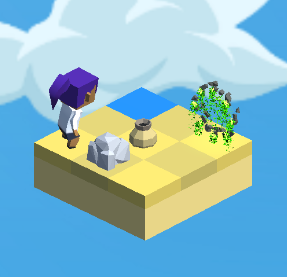
\includegraphics{pic/prefabs.png}
\end{center}
\caption[ตัวอย่าง prefabs ที่ใช้]{ตัวอย่าง prefabs ที่ใช้ }
\label{prefabs}
\end{figure}

\chapter{\ifproject%
\ifcpe โครงสร้างและขั้นตอนการทำงาน\else Project Structure and Methodology\fi
\else%
\ifcpe โครงสร้างของโครงงาน\else Project Structure\fi
\fi
}

% ในบทนี้จะกล่าวถึงหลักการ และการออกแบบระบบ

\makeatletter

% \renewcommand\section{\@startsection {section}{1}{\z@}%
%                                    {13.5ex \@plus -1ex \@minus -.2ex}%
%                                    {2.3ex \@plus.2ex}%
%                                    {\normalfont\large\bfseries}}

\makeatother
%\vspace{2ex}
% \titleformat{\section}{\normalfont\bfseries}{\thesection}{1em}{}
% \titlespacing*{\section}{0pt}{10ex}{0pt}

\section{Model View Controller (MVC)}
โครงงานนี้ใช้ design pattern MVC~\cite{mvc}\CIreply{ทำไมเป็นคำว่า ``และ''}แบ่งออกเป็น 3 ส่วนหลักๆ ดังรูปที่ \ref{mvc} คือ 
\begin{enumerate}
    \item Model
    \item View
    \item Controller
\end{enumerate}

\begin{figure}
\begin{center}
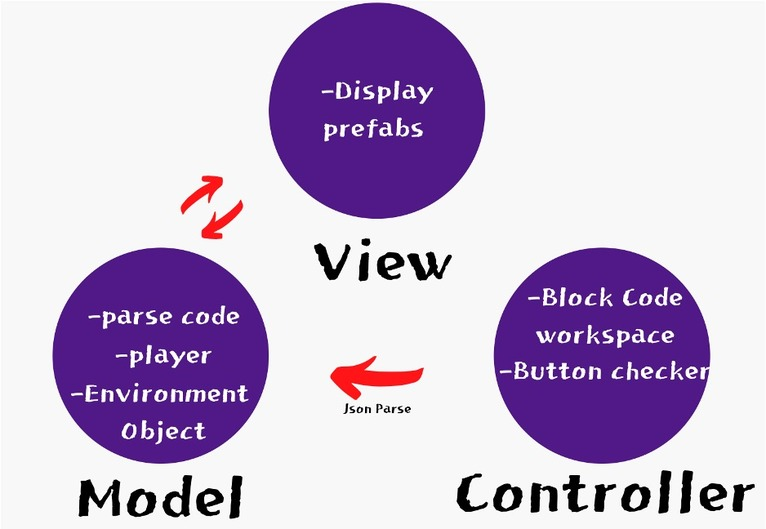
\includegraphics{pic/pic1.jpg}
\end{center}
\caption[Poem]{Design Pattern MVC}
\label{mvc}
\end{figure}

\subsection{Model}
 ในส่วนของ Model จะเป็นการจัดการแปลงจาก Block Code ให้เป็น C\# เพื่อทำให้เกิด Event ต่างๆ เช่นการเดิน, การหมุน
 และการกระโดด เป็นต้น โดยที่ Model จะรับBlock Code มาจาก Controller ในรูปของ JSON
 และจะทำการแปลงเป็น C\# เพื่อสั่งให้ view แสดงผลต่างๆ ส่วนของ Model จะอยู่ใน Unity
 เป็นตัวกลางในการสื่อสารระหว่าง View กับ Controller

\subsection{View}
View นั้นทำหน้าที่แค่แสดงผลโดยรับโค้ดคำสั่งมาจาก Model และทำการแสดงผล จากนั้นจะทำการ
ส่งค่าคืน เพื่อบอก Model ว่าแสดงผลตามตามคำสั่งนั้นแล้ว ในส่วนของ View นั้นจะอยู่ใน
Unity เช่นกัน เพราะ View ใช้แสดงผลกราฟฟิกของ Unity ที่ผู้พัฒนาได้สร้างเอาไว้ เช่น prefabs(รูปแบบสำเร็จ) ต่างๆ ดังรูปที่ \ref{prefabs}
รวมไปถึงการแสดงหน้า UI ของเกม ซึ่งจะกล่าวถึงในหัวข้อ User Interface\par

\begin{figure}
    \begin{center}
    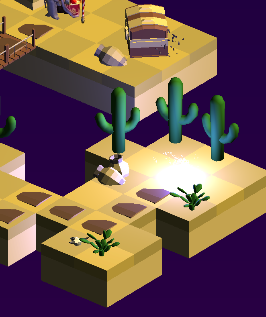
\includegraphics{pic/prefap.PNG}
    \end{center}
    \caption[Poem]{ตัวอย่าง prefabs ที่ใช้ }
    \label{prefabs}
    \end{figure}
    


\subsection{Controller}
Controller จะอยู่ทั้ง 2 ฝั่ง คือทั้ง Unity และ WebView โดย Controller ฝั่งหน้าเว็ปจะเป็นการรอให้ผู้ใช้
ลากวางตัว Block Code และเมื่อผู้ใช้กดรัน Controller ฝั่งหน้าเว็ปจะทำการแปลง Block Code ให้เป็น Object 
ในรูปของ JSON และจะถูกนำส่งไปให้ Controller ฝั่ง Unity หลักจากนั้น Controller ฝั่ง Unity จะทำการ
ประมวลผลและแปลงเป็น Object ที่ Unity สามารถอ่านได้เพื่อส่งต่อไปให้ Model

\section{User Interface (UI)}
User interface (UI) คือ การออกแบบที่เน้นไปที่เรื่องหน้าตา ความสวยงาม และทุกอย่างที่จะเป็นการโต้ตอบกับผู้ใช้งาน UI ที่ดีจะช่วยดึงดูดผู้ใช้งานให้เกิดความสนใจและช่วยให้ผู้ใช้งานเข้าถึงข้อมูลได้ง่าย
โดยการออกแบบ UI ของเกมนี้พวกเราจะออกแบบเกมแนวตะลุยอวกาศ โดยจะใช้ Asset ที่มีอยู่ใน Unity มาปรับแต่งจัดวางเพื่อความสวยงามและความน่าสนใจ โดยจะมีส่วนต่างๆ ดังนี้ ซึ่งจะแสดงดังรูปต่อไปนี้
\begin{itemize}
\item หน้าจอแสดง Mainmenu รูปที่ \ref{mainmenu}
\item หน้าจอแสดงหน้าเลือกด่าน รูปที่ \ref{stage}
\item หน้าต่างแสดงเมนูการตั้งค่า รูปที่ \ref{setting}
\item หน้าจอแสดงหน้า Gameplay รูปที่ \ref{game}
\item หน้าต่างที่แสดงว่าเราชนะ รูปที่ \ref{win}
\item หน้าต่างที่แสดงว่าเราแพ้ รูปที่ \ref{lose}
\end{itemize}


\begin{figure}
\begin{center}
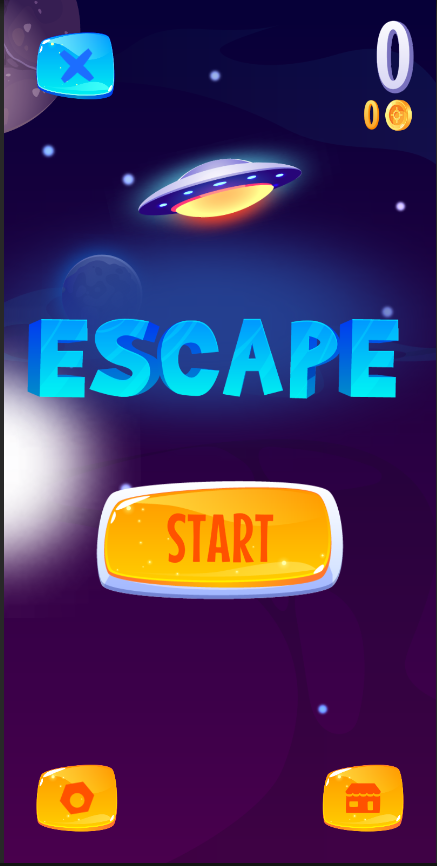
\includegraphics[scale = 0.4]{pic/home_start.PNG}
\end{center}
\caption[Poem]{หน้า Mainmenu ของเกม}
\label{mainmenu}
\end{figure}

\begin{figure}
\begin{center}
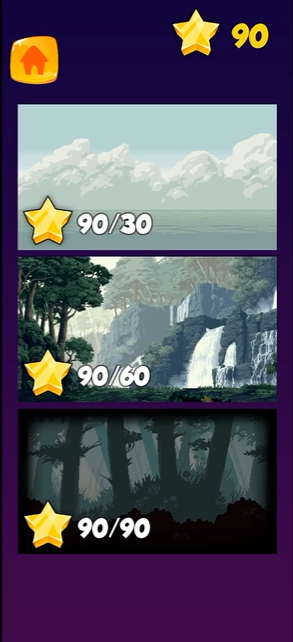
\includegraphics[scale = 0.4]{pic/MapSelection.png}
\end{center}
\caption[Poem]{หน้าเลือกด่าน}
\label{stage}
\end{figure}

\begin{figure}
\begin{center}
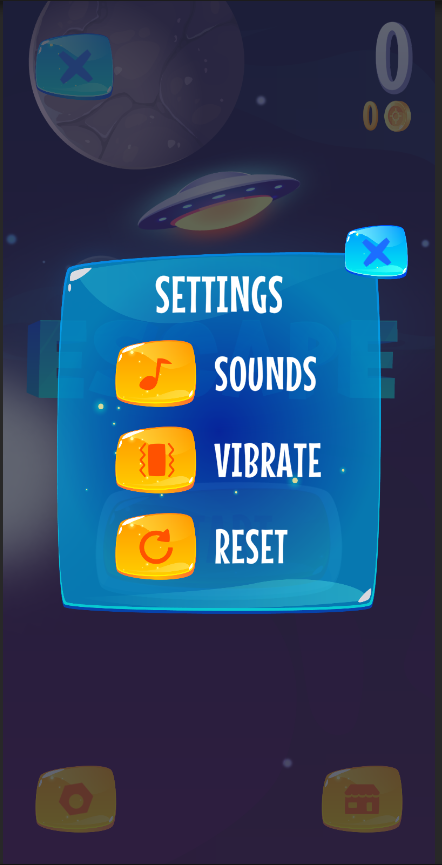
\includegraphics[scale = 0.4]{pic/setting.PNG}
\end{center}
\caption[Poem]{เมนูการตั้งค่า}
\label{setting}
\end{figure}

\begin{figure}
\begin{center}
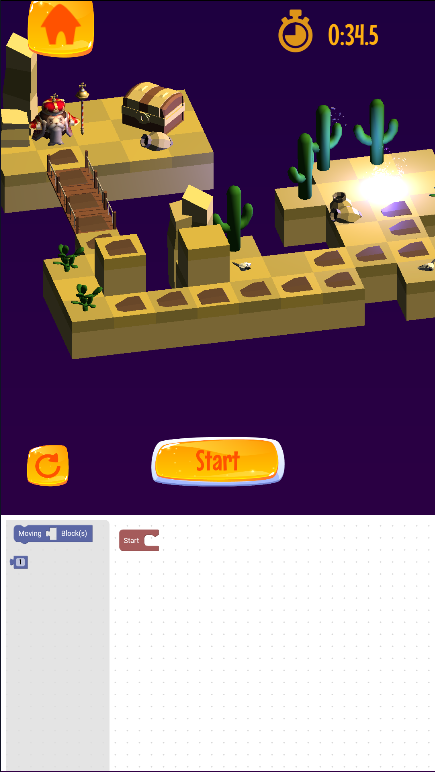
\includegraphics[scale = 0.4]{pic/gameplay.PNG}
\end{center}
\caption[Poem]{หน้า Gameplay}
\label{game}
\end{figure}

\begin{figure}
\begin{center}
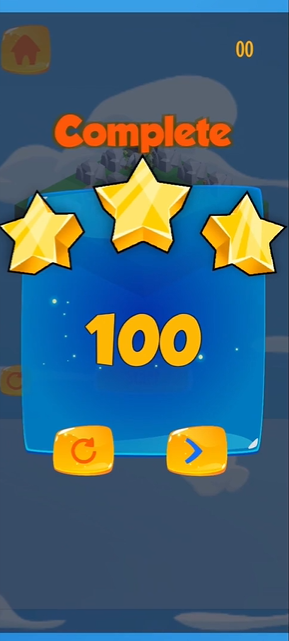
\includegraphics[scale = 0.4]{pic/Complete.png}
\end{center}
\caption[Poem]{หน้าต่างที่แสดงว่าชนะ}
\label{win}
\end{figure}

\begin{figure}
\begin{center}
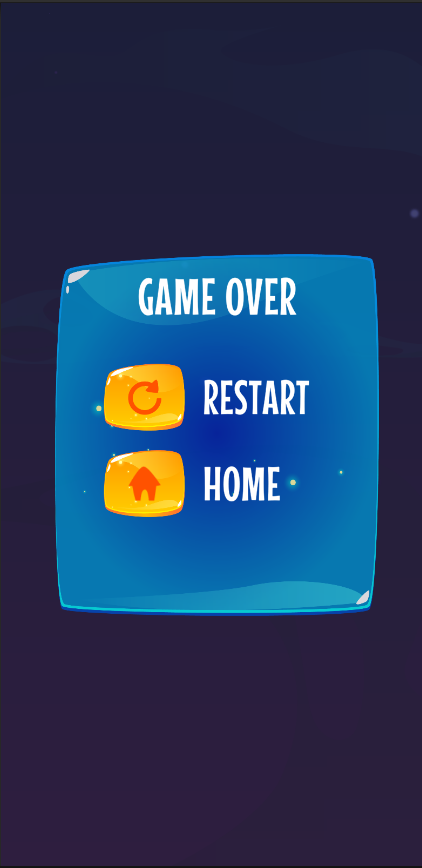
\includegraphics[scale = 0.4]{pic/gameover.PNG}
\end{center}
\caption[Poem]{หน้าต่าง GameOver}
\label{lose}
\end{figure}



\section{WebView}
ตัวหน้าเว็ปทำขึ้นมาเพื่อนำ Google Blockly ไปใส่ใน panel ของ Unity เพราะเดิมที Unity ไม่สามารถสร้าง Object ที่หน้าตาและรวมไปถึง function ที่เหมือนกับ Google Blockly ได้ ทางผู้พัฒนาเลยสร้างหน้าเว็ปเข้ามาเพื่อนำไปใส่ใน 
panel ของ Unity ที่ใช้ในการแสดงผล Block Code


\begin{figure}
\begin{center}
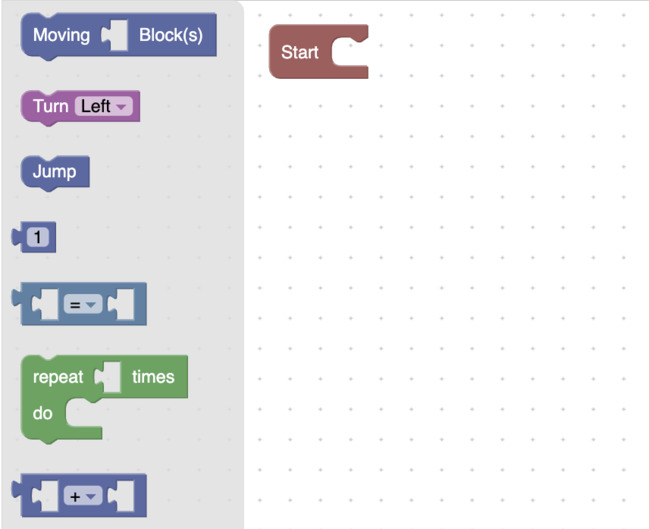
\includegraphics{pic/block1.jpg}
\end{center}
\caption[Poem]{Google Blockly}
\label{block}
\end{figure}

\section{Text Reader}
การสร้างด่านของเกมนี้จะ Input ด้วยไฟล์ Text กล่าวคือเมื่อ User ทำการ Input ไฟล์มาตัวระบบเกมจะทำการจัดการสร้างด่านให้เอง
ทำให้การที่จะสร้างด่านหนึ่งด่านไม่ต้องทานั่งลากวางตัว prefabs บน Unity ตัวอย่างไฟล์ Text คร่าวๆ จากรูป\ref{txt}
\begin{figure}
    \begin{center}
    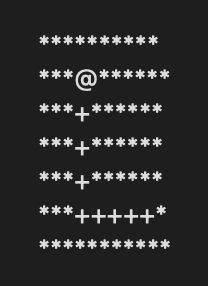
\includegraphics{pic/text.png}
    \end{center}
    \caption[Poem]{Text}
    \label{txt}
    \end{figure}

\chapter{\ifproject%
\ifcpe การทดลองและผลลัพธ์\else Experimentation and Results\fi
\else%
\ifcpe การประเมินระบบ\else System Evaluation\fi
\fi}

% ในบทนี้จะทดสอบเกี่ยวกับการทำงานในฟังก์ชันหลักๆ
% การทดสอบระบบของเราจะทดสอบโดยใช้ User Test ซึ่งเราจะนำไปให้กลุ่มทดลองที่เป็นเด็กนักเรียนชั้นประถมศึกษาปีที่ 4-6 โรงเรียนรอบนอก
% ชั้นปีละ 20 คนในการทดสอบโดย เราจะวัดผลโดยการใช้ pre-test เพื่อวัดระดับของเด็กนักเรียนก่อนเล่นเกมและ post-test เพื่อวัดระดับของเด็กนักเรียนหลังเล่นเกม
% ซึ่งในเนื้อหา pre-test และ post-test จะเป็นแบบฝึกหัดเนื้อหาวิชาวิทยาการคำนวณ โดยเราจะนำผล pre-test และ post-test มาเทียบกันเพื่อ
% ประเมินตัวเกมของเราว่าจะสามารถเป็นสื่อการเรียนการสอนให้เด็กนักเรียนได้เข้าใจในวิชาวิทยาการคำนวณมากขึ้นจริงไหม 
% รวมไปถึงภายในตัวเกมเองก็จะมีการเก็บ Score ของผู้เล่นโดยแต่ละด่านจะมีจำนวณจำกัดในการใช้ Block Code ซึ่งถ้านักเรียนใช้จำนวณคำสั่งเกินมาจากที่กำหนดไว้คะแนนของนักเรียนจะ
% ลดลงตามจำนวณคำสั่งที่เพิ่มมาและจะมีการเก็บเวลาที่ใช้ในแต่ละด่านของนักเรียนแต่ละคนเดียว ทั้งหมดนี้จะนำไปขึ้น Score Board เพิ่งแสดงให้เห็นว่าตัวนักเรียนเองได้คะแนนจากด่านนี้ๆ เท่าไหร่
% \CIreply{ใจความของย่อหน้านี้คืออะไร
การประเมินระบบของโครงการนี้ จะมีการประเมิณอยู่ 2 วิธีคือ User Test ซึ่งจะเป็นเด็กนักเรียนชั้นประถมศึกษาปีที่ 3-6 โดยผ่านเครื่องมือการ Pre-Test
Post-Test และอีกวิธีคือ Expert Test เป็นการประเมินประเมินระบบภายในเกม ความยากง่ายของเกม (Game Design) และ UX/UI ผ่าน
เครื่องมือที่เรียกว่า IOC

\section{User Test}
การศึกษาเรื่องการวัดผลวิชาวิทยาการคำนวณสำหรับนักเรียนชั้นประถมศึกษาปีที่ 3 – 6 
โรงเรียนบ้านออนใต้และโรงเรียนบ้านโฮ้ง อำเภอสันกำแพง
 จังหวัดเชียงใหม่ โดยใช้การวัดผลแบบ Pre-test Post-test ก่อนและหลังเล่นเกม ผู้ศึกษานำเสนอผลวิเคราะห์ข้อมูลตามลำดับดังนี้
\subsection{Pre-test Post-test}
ผลสัมฤทธิ์ทางการเรียนรู้เรื่องวิชาวิทยาการคำนวณหมวดการคิดอย่างเป็นขั้นเป็นตอบโดยใช้เกมเสริมทักษะวิชาวิทยาการคำนวณ (Escape) ของนักเรียนชั้นประถมศึกษาปีที่ 3 – 6
โรงเรียน บ้านออนใต้และโรงเรียนบ้านโฮ้ง อำเภอสันกำแพง จังหวัดเชียงใหม่\par
ได้สร้างเกมเสริมทักวิชาวิทยาการคำนวณสำหรับนักเรียนชั้นประถมศึกษาปีที่ 3 – 6 โรงเรียน
บ้านออนใต้และโรงเรียนบ้านโฮ้ง อำเภอสันกำแพง จังหวัดเชียงใหม่ จำนวน 1 เกม
โดยภายในเกมประกอบไปด้วยด่านจำนวน 30 ด่าน
แต่ละด่านประกอบไปด้วยรายละเอียดดังต่อไปนี้\par
\begin{center}
    \begin{tabular}{|c | m{35em}|} 
     \hline
     ด่านที่ & เนื้อหา\\ [0.5ex] 
     \hline\hline
     1 &  ศึกษาวิธีการเล่นเกมโดยให้ตัวละครเดินไป 1 ก้าว \\ 
     \hline
     2 &  ศึกษาวิธีการเปลี่ยนค่าในกล่องคำสั่งโดยให้ตัวละครเดินไป 2 ก้าว \\ 
     \hline
     3 &  ศึกษาวิธีการเปลี่ยนค่าในกล่องคำสั่งโดยให้ตัวละครเดินไป 4 ก้าว \\ 
     \hline
     4 &  ศึกษาคำสั่งใหม่ (หมุน) โดยให้ตัวละครหมุน 1 ครั้งและเดิน 1 ก้าว \\ 
     \hline
     5 &  ศึกษาคำสั่งใหม่ (หมุน) โดยให้ตัวละครหมุน 1 ครั้งและเดิน 4 ก้าว \\ 
     \hline
     6 &  ผสมผสานคำสั่งโดยให้ตัวละครเดินและหมุน \\ 
     \hline
     7 &  ผสมผสานคำสั่งโดยให้ตัวละครเดินและหมุนไปในอีกทิศทาง \\ 
     \hline
     8 &  เพิ่มระดับความยากจากด่านก่อนหน้าโดยต้องใช้คำสั่ง หมุนและเดิน มากขึ้น \\ 
     \hline
     9 &  เพิ่มระดับความยากจากด่านก่อนหน้าโดยต้องใช้คำสั่ง หมุนและเดิน มากขึ้น \\ 
     \hline
     10 &  เพิ่มระดับความยากจากด่านก่อนหน้าโดยต้องใช้คำสั่ง หมุนและเดิน มากขึ้น \\ 
     \hline
     11 &  ศึกษาคำสั่งใหม่ (ทำซ้ำ) โดยให้ผู้ใช้เดินไป 1 ด้าวและครอบด้วยคำสั่งทำซ้ำไ \\ 
     \hline
     12 &  ผสมผสานคำสั่ง เดิน,หมุน และทำซ้ำโดยให้ตัวละครเดินเป็นตัว U คว่ำ \\ 
     \hline
     13 &  ผสมผสานคำสั่ง เดิน,หมุน และทำซ้ำโดยให้ตัวละครเดินเป็นซิกเซ็ก \\ 
     \hline
     14 &  ผสมผสานคำสั่ง เดิน,หมุน และทำซ้ำโดยให้ตัวละครเดินเป็นตัว U คว่ำที่ใหญ่กว่า \\ 
     \hline
     15 &  ผสมผสานคำสั่ง เดิน,หมุน และทำซ้ำโดยให้ตัวละครเดินเป็นตัว U คว่ำ โดยมีการหลอก \\ 
     \hline
     16 &  ศึกษาคำสั่งใหม่ (ตัวแปร) \\ 
     \hline
     17 &  ศึกษาวิธีเปลี่ยนค่าของคำสั่งตัวแปร \\ 
     \hline
     18 &  ผสมผสานคำสั่ง เดิน,ตัวแปร และหมุน \\ 
     \hline
     19 &  ผสมผสานคำสั่ง เดิน,ตัวแปร,หมุน และทำซ้ำโดยให้ตัวละครเดินเป็นรูปเปลือกห้อง \\ 
     \hline
     20 &  ผสมผสานคำสั่ง เดิน,ตัวแปร,หมุน และทำซ้ำโดยให้ตัวละครเดินเป็นรูปเปลือกห้องที่ใหญ่ขึ้น \\ 
     \hline
     21 &  ศึกษาคำสั่งใหม่ (เหยียบบน Block สี) โดยให้เดินไปข้างหน้า \\ 
     \hline
     22 &  ผสมผสานคำสั่ง เดิน, หมุน และเหยียบบน Block สี \\ 
     \hline
     23 &  ผสมผสานคำสั่ง เดิน, หมุน และเหยียบบน Block สีโดยมีการเปลี่ยนค่าของคำสั่ง \\ 
     \hline
     24 &  ผสมผสานคำสั่ง เดิน, หมุน, เหยียบบน Block สี และ ทำซ้ำ \\ 
     \hline
     25 &  ผสมผสานคำสั่ง เดิน, หมุน, เหยียบบน Block สี และ ทำซ้ำ โดยให้เดินเป็นรูปตัว U คว่ำ \\ 
     \hline
     26 &  เพิ่มจำนวน Block สีที่เหยียบได้ โดยในด่านจะมี 2 สี \\ 
     \hline
     27 &  ผสมผสานคำสั่ง เดิน, หมุน, เหยียบบน Block สี และ ทำซ้ำ โดยให้เดินเป็นซิกเซ๊ก \\ 
     \hline
     28 &  ผสมผสานคำสั่ง เดิน, หมุน, เหยียบบน Block สี และ ทำซ้ำ โดยให้เดินเป็นซิกเซ๊กโดยเพิ่มจำนวนคำสั่งที่ใช้ \\ 
     \hline
     29 &  ผสมผสานคำสั่ง เดิน, หมุน, เหยียบบน Block สี และ ทำซ้ำ โดยให้เดินเป็นรูปตัว U คว่ำพร้อมทั้งมีการหลอกการใช้คำสั่ง \\ 
     \hline
     30 &  ผสมผสานคำสั่ง เดิน, หมุน, เหยียบบน Block สี และ ทำซ้ำ โดยมี Block สีที่เหยียบได้ 3 สี \\ 
     \hline
    \end{tabular}
\end{center}

จากผลการประเมินความเหมาะสมของเกมเสริมทักษะวิชาวิทยาการคำนวณ (Escape) สำหรับนักเรียนชั้นประถมศึกษาปีที่ 
3 – 6 โรงเรียน บ้านออนใต้และโรงเรียนบ้านโฮ้ง อำเภอสันกำแพง จังหวัดเชียงใหม่ 
โดยมีผู้เชี่ยวชาญจำนวน 2 ท่านปรากฏผลดังนี้ ได้ปรับแก้เนื้อหาที่อิงตามหลักสูตรวิชาวิทยาการคำนวณภายในด่าน 
ให้เหมาะสมกับศักยภาพและวัยของผู้เรียน และเมื่อนำเกมเสริมทักษะวิชาวิทยาการคำนวณ (Escape) 
ไปใช้กับกลุ่มเป้าหมายพบประเด็นที่น่าสนใจดังนี้

\begin{enumerate}
    \item นักเรียนมีความกระตือรือร้นในการทำกิจกรรมโดยใช้เกมเสริมทักษะวิชาวิทยาการคำนวณ (Escape) และได้รับสนุกสนานควบคู่ไปกับความรู้ 
    \item เสริมสร้างกระบวนการเรียนรู้ทางเทคโนโลยีและฝึกให้เด็กได้ใช้ความคิดอย่างเป็นขั้นเป็นตอนตามหลักสูตรแกนกลางการศึกษาขั้นพื้นฐานพุทธศักราช 2560 ในรายวิชาวิทยาศาสตร์ (วิทยาการคำนวณ)
\end{enumerate}
ผลการเรียนรู้เรื่องวิชาวิทยาการคำนวณสำหรับนักเรียนชั้นประถมศึกษาปีที่ 3 – 6 โรงเรียน บ้านออนใต้และโรงเรียนบ้านโฮ้ง อำเภอสันกำแพง จังหวัดเชียงใหม่\par
คะแนนจากการทำแบบทดสอบวัดผลการเรียนรู้ของวิชาวิทยาการคำนวณหมวดหมู่การคิดอย่างเป็นขั้นเป็นตอน โดยใช้เครื่องมือคือเกมเสริมทักษะวิชาวิทยาการคำนวณ (Escape)\par
\bigskip

\begin{tikzpicture}

    \begin{axis} [
        xtick={ป.3,ป.4,ป.5,ป.6},  % Use this to decide which tickmarks to print
        xticklabel style={text height=2ex}, % This aligns all letters on the same line, if it is missing, 'a' and 'b' are at different heights
        ymin=0,
        ylabel=คะแนน,
        ymin=0,
        symbolic x coords={ป.3,ป.4,ป.5,ป.6},
        legend style={at={(0.5,-0.1)},
        anchor=north,legend columns=-5},
        width=11cm,
        ybar,
        bar width=7pt,
    ]
     
    \addplot[red!20!black,fill=red!80!white,ybar,fill] coordinates {(ป.3,34) (ป.4,38) (ป.5,67) (ป.6,73)};
    \addplot[blue!20!black,fill=blue!80!white,ybar,fill] coordinates {(ป.3,32) (ป.4,40) (ป.5,84) (ป.6,100)};

    \legend {Pre-Test, Post-Test};
     
    \end{axis}
     
\end{tikzpicture}\bigskip

จากการทดสอบนักเรียนชั้นประถมศึกษาชั้นปีที่ 3 - 6 ด้วยข้อสอบวิชาวิทยาการคำนวณก่อนและหลังเล่นเกม นักเรียนทุกคนมีพัฒนาการเพิ่มขึ้นเป็นที่น่าพึงพอใจเมื่อทำ
ข้อสอบที่มีความยากมากขึ้น


\section{Expert test}
การประเมินในด้านระบบของเกมโดยใช้ผู้เชี่ยวชาญในการประเมินคุณภาพอุปกรณ์(เกมเสริมทักษะวิชาวิทยาการคำนวน) จำนวน 3 ท่าน มีหัวข้อการประเมินประกอบไปด้วย UX/UI ของเกม, ความยากง่ายของเกมเมื่อเทียบกับผู้ใช้ซึ่งก็คือนักเรียนชั้นประถม
ศึกษาปีที่ 3 - 6, ผลที่คาดว่าจะสามารถเพิ่มทักษะกาาคิดอย่างเป็นขั้นเป็นตอนให้กับเด็ก และระบบของเกมโดยรวมประกอบไปด้วย 
การลื่นไหลของ animation, ความเร็วการตอบสอนของเกม (ไม่มี delay), ไม่เจอ error ของระบบ (เด้งหรือค้าง) โดยใช้
โดยทางผู้พัฒนาได้ใช้ model IOC ในการทดสอบวัดคุณภาพของเครื่องมือ(เกมเสริมทักษะวิชาวิทยาการคำนวน) ซึ่งผู้เชี่ยวชาญจะ
ประเมินแต่ละหัวข้อด้วย 3 ตัวเลือกซึ่งก็คือ ผ่าน, ไม่ทราบ, ไม่ผ่าน โดยที่ในแต่ละหัวข้อจะสามารถผ่านได้เมื่อค่าเฉลี่ยในการ
เลือกให้ผ่านเป็นค่า 66.7\%-symbol กล่าวคือในแต่ละหัวข้อต้องถุกประเมินให้ผ่าน 2 ใน 3 ของจำนวนผู้เชี่ยวชาญ โดยมีผลลัพธ์ดังนี้
\begin{center}
    \begin{tikzpicture}
        \pie[text = legend]{100 / ผ่าน}
    \end{tikzpicture}
\end{center}
ความเหมาะสมทางด้าน UX
\begin{center}
    \begin{tikzpicture}
        \pie[text = legend]{66.7 / ผ่าน, 33.3 / ไม่ทราบ}
    \end{tikzpicture}
\end{center}
ความเหมาะสมทางด้าน UI
\begin{center}
    \begin{tikzpicture}
        \pie[text = legend]{100 / ผ่าน}
    \end{tikzpicture}
\end{center}
นักเรียนชั้นประถมศึกษาชั้นปีที่ 3 - 6 สามารถเล่นเกมนี้ได้
\begin{center}
    \begin{tikzpicture}
        \pie[text = legend]{100 / ผ่าน}
    \end{tikzpicture}
\end{center}
ตัวเกมสามารถช่วยเพิ่มทักษะการคิดอย่างเป็นขั้นเป็นตัวให้กับเด็กนักเรียนได้
\begin{center}
    \begin{tikzpicture}
        \pie[text = legend]{66.7 / ผ่าน, 33.3 / ไม่ทราบ}
    \end{tikzpicture}
\end{center}
ตัวระบบโดยรวมของเกม การลื่นไหลของ animation , ความเร็วการตอบสอนของเกม (ไม่ delay) , ไม่เจอ error ของระบบ (เกมเด้ง/ค้าง)



\ifproject
\chapter{\ifcpe บทสรุปและข้อเสนอแนะ\else Conclusions and Discussion\fi}

\section{\ifcpe สรุปผล\else Conclusions\fi}
% ทางผู้พัฒนาได้เล็งเห็นถึงความสำคัญของวิชาวิทยาการคำนวณเลยได้ศึกษาวิชาวิทยาการคำนวณซึ่งเป็นวิชาล่าสุดที่ถูกนำมาเพิ่มในรายวิชาวิทยาศาสตร์ในปี พศ. 2560 โดยหลักๆ ในตัวรายวิชาจะเป็นเกี่ยวกับ
% เทคโนโลยี ประกอบไปด้วย การเขียนโปรแกรม, การใช้เทคโนโลยี, การมีภูมิคุ้มกันต่อเทคโนโลยี, การพัฒนาทักษะการคิดอย่างเป็นขั้นเป็นตอน, ฯลฯ
% และเมื่อลงพื้นที่เพื่อไปศึกษาวิชาวิทยาการคำนวณ ณ โรงเรียนบ้านดอยเต่าซึ่งเป็นโรงเรียนรอบนอก ทำให้เราได้เล็งเห็นปัญหาของตัวเด็กนักเรียนเกี่ยวกับวิชาวิทยาการคำนวณ นั่นก็คือ
% การที่ตัวเด็กนักเรียนเองไม่สามามรถเรียนรู้วิชาวิทยาการคำนวณได้เต็มที่ในหลายๆ ปัจจัยที่เกี่ยวข้อง เช่นการที่เด็กไม่ชอบเรียนวิชาวิทยาการคำนวณ
% เพราะว่าไม่มีครูสอนหรือรวมไปถึงตัวเด็กเองไม่ได้ตั้งใจเรียนอยู่แล้ว ทำให้เกิดโครงงานนี้มาเพื่อเป็นสื่อและเครื่องมือผ่านเกมที่เป็น Mobile เกมผ่านโทรศัพท์มือถือเพื่อการพัฒทักษะวิชาวิทยาการคำนวณ
% โดยที่ผู้พัฒนาจะมุ่งเน้นไปที่ทักษะการคิดอย่างเป็นขั้นเป็นตอนซึ่งเป็นทักษะที่สำคัญในการแก้ไขปัญหาต่างๆ
% โครงงานนี้มีจุดประสงค์ดังต่อไปนี้คือ ลดความเหลื่อมล้ำทางด้านการศึกษา, ทำให้เด้กนักเรียนสามารถนำความรู้ที่ได้ไปแก้ไขปัญหาในชีวิตประจำวันได้ และ
% ผลักดันหลุกสูตรวิชาวิทยาการคำนวณ เนื้อหาในตัวเกมที่ผู้พัฒนาสร้างขึ้นจะเน้นไปที่การพัฒนาทักษะการคิดอย่างเป็นขั้นเป็นตอน
% ซึ่งผู้พัฒนาจะอิงตามหลักสูตรวิชาวิทยาการคำนวณของ สสวท. โดยเนื้อหาในตัวเกมนั้นจะเป็นในรูปแบบของการแก้ไขปริศนากล่าวคือ ผู้เล่น(เด็กนักเรียน)
% ต้องแก้ปริศนาคือการให้ตัวละครในเกมเดินไปยังจุดหมายหรือเส้นชัยผ่านการเลือกวาง Blockly Code ซึ่งรูปแบบของด่านในเกม
% จะอิงตามหนังสือวิชาวิทยาการคำนวณของ สสวท. โดยผู้พัฒนาได้แบ่งการทดสอบเป็น 2 อย่าง คือการทดสอบกับกลุ่มตัวอย่างซึ่งก็คือนักเรียนชั้นประถมศึกษาปีที่ 3-6 จำนวน 71 คนเพื่อทดสอบ
% ว่าเครื่องมือหรือเกมเสริมทักษะวิชาวิทยาการคำนวณนั้นสามารถเสริมทักษะวิชาวิทยาการคำนวณได้จริงผ่านการทดสอบ pre-test, post-test โดยข้อสอบจะอิงตามหนังสือวิชาวิทยาการคำนวณของ สสวท. ซึ่งผลที่ได้ออกมาคือนักเรียนทุกคนนั้นมีพัฒนาการหลังจากการ
% เล่นเกมเสริมทักษะวิชาวิทยาการคำนวณ เนื่องจากโครงงานนี้เป็นการสร้างซอฟแวร์ซึ่งเป็นในรูปแบบของเกมทำให้ต้องมีการทดสอบระบบต่างๆ ซึ่งประกอบไปด้วย UX, UI, เนื้อหาในเกม, ลำดับความยากง่ายของด่านต่อไป เป็นต้น ดังนั้น
% ทางผู้พัฒนาเลยมีการทดสอบตัวระบบของเกมเสริมทักษะวิชาวิทยาการคำนวณผ่านผู้เชี่ยวชาญจำนวน 3 ท่านซึ่งมีประสบการทางด้านการเขียนโปรแกรมผ่าน Unity ไม่ต่ำกว่า 3 ปี โดยผู้พัฒนาใช้โมเดล IOC ในการวัดผลและผลที่ออกมา
% คือทุกหัวข้อในการทดสอบผ่านทั้งหมด ดังนั้นจึงสรุปได้ว่าโครงงานเกมเสริมทักษะวิชาวิทยาการคำนวณนั้นสามารถลดความเหลื่อมล้ำทางด้านการศึกษากล่างคือ หลังจากนักเรียนได้เล่นเกมเสริมทักษะวิชาวิทยาการคำนวณไป
% นักเรียนสามารถทำข้อสอบวิชาวิทยาการคำนวณที่อิงจากหนังสือ สสวท. ได้ซึ่งไม่ต่างกับเด็กนักเรียนที่เรียนตามหนังสือวิชาวิทยาการคำนวณของ สสวท. 
% นอกจากนี้นักเรียนเองสามารถนำความรู้ไปแก้ไขปัญหาในชีวิตจริงได้กล่าวคือ ใน post-test ทางผู้พัฒนาได้เพิ่มความลึกของข้อสอบโดย
% เพิ่มการคิดต่อยอดเข้าไปซึ่งตัวเด็กนักเรียนเองก็สามารถทำได้ หลังจากที่ผู้พัฒนาได้เข้าไปลงพื้นที่เพื่อทดสอบเกมเสริมทักษะวิชาวิทยาการคำนวณกับกลุ่มตัวอย่างทำให้ทางโรงเรียนที่ไปลงพื้นที่นั้น
% สนใจในเกมเสริมทักษะวิชาวิทยาการคำนวณเป็นอย่างมากอละได้เล็งเห็นถึงความสำคัญของหลักสูตรวิชาวิทยาการคำนวณซึ่งเป็นการผลักดันหลักสูตรวิชาวิทยาการคำนวณตามที่ผู้พัฒนาได้ตั้งไว้
จากผลการทดสอบจากบทที่ \ref{eval} เกมเสริมทักษะวิชาวิทยาการคำนวณเป็นเกมที่สามารถเพิ่มทักษะการคิดเชิงคำนวณและการคิดอย่างเป็นขั้นเป็นตอนได้ดีเยี่ยม สมควรเป็นอย่างยิ่งที่จะพัฒนาต่อ
ซึ่งบรรลุจุดประสงค์ที่ได้ตั้งไว้ กล่าวคือ การลดความเหลือมล้ำทางด้านการศึกษา โดยหลังจากนักเรียนได้เล่นเกมเสริมทักษะวิชาวิทยาการคำนวณไปแล้ว นักเรียนสามารถทำข้อสอบวิชาวิทยาการคำนวณที่อิงจากหนังสือ สสวท. ได้ไม่ต่างกับเด็กนักเรียนที่เรียนตามหนังสือวิชาวิทยาการคำนวณของ สสวท. 
นอกจากนี้ นักเรียนเองสามารถนำความรู้ไปแก้ไขปัญหาในชีวิตจริงได้ กล่าวคือ ใน post-test ทางผู้พัฒนาได้เพิ่มความลึกของข้อสอบ โดยเพิ่มการคิดต่อยอดเข้าไป ซึ่งตัวเด็กนักเรียนเองก็สามารถทำได้ 

หลังจากที่ผู้พัฒนาได้เข้าไปลงพื้นที่เพื่อทดสอบเกมเสริมทักษะวิชาวิทยาการคำนวณกับกลุ่มตัวอย่าง ทำให้ทางโรงเรียนที่ไปลงพื้นที่นั้นสนใจในเกมเสริมทักษะวิชาวิทยาการคำนวณเป็นอย่างมาก และได้เล็งเห็นถึงความสำคัญของหลักสูตรวิชาวิทยาการคำนวณ ซึ่งเป็นการผลักดันหลักสูตรวิชาดังกล่าว ตามที่ผู้พัฒนาได้ตั้งมั่นไว้

สุดท้ายนี้ โครงงานหนีจากวังวน (Escape) เกมเสริมทักษะวิชาวิทยาการคำนวณนี้ สามารถนำไปใช้ในการพัฒนาทักษะวิชาวิทยาการคำนวณ และการคิดอย่างเป็นขั้นเป็นตอนของเด็กนักเรียนได้อย่างมีประสิทธิภาพ


\section{\ifcpe ปัญหาที่พบและแนวทางการแก้ไข\else Challenges\fi}

ในการทำโครงงานนี้ พบว่าเกิดปัญหาหลักๆ อยู่ 2 ส่วน ดังนี้

\subsection{ปัญหาทางด้านเครื่องมือสร้างเกม (Unity)}
เกมเสริมทักษะวิชาวิทยาการคำนวณที่ได้พัฒนาขึ้นมานั้น เป็นเกมที่ไม่เหมือนเกมทั่วไปที่สร้างด้วย
Unity โดยตัวเกมหลักๆ จะประกอบไปด้วยกันอยู่ 2 ส่วนคือส่วนที่เป็น Unity แสดงผลต่างๆ และหน้าเว็บ ซึ่งทางหน้าเว็บผู้พัฒนาต้องเก็บไว้ในตัว resources file
บน Unity และเมื่อเริ่มการ build โปรเจคที่โครงสร้างไฟล์ต่างจากปกติ ทำให้ Gradle linker ทำงานผิดพลาด ดังนั้น ผู้พัฒนาจึงต้องทำการ manual link ไฟล์ต่างๆ เอง
ซึ่งเป็นส่วนที่ทำให้เสียเวลาในการพัฒนาตัวเกมมาก

\subsection{ปัญหาระหว่างการทดสอบกับกลุ่มตัวอย่าง}
ปัญหาระหว่างการทดสอบ แบ่งได้ออกเป็น 2 หัวข้อ ดังนี้
% \subsubsection{เมื่อทดสอบกับกลุ่มตัวอย่างสิ่งที่เรียกว่าบัคนั้นได้เกิดขึ้นจากการเขียนโปรแกรมของทางผู้พัฒนา เช่น เดิมตกแมพ, ตัวละครบินได้, ตัวแสดงผลหน้าเว็ปนั้นค้าง ซึ่งได้รับการแก้ไข้หลังจากไปทดสอบกับกลุ่มตัวอย่างเสร็จแล้ว}
% \subsubsection{การเข้าไปทดสอบในช่วงที่มีโรคระบาด Covid-19 ทำให้มีอุปสรรคเช่น การเข้าใกล้ชิดกับนักเรียนและการรวมกลุ่มกันของนักเรียน ทำให้ต้องมีขั้นตอนในการปฎิบัติตามมาตรการป้องกันคือ การตรวจหาเชื้อ Covid-19 ก่อนเข้าไปทดสอบกับกลุ่มตัวอย่างและต้องทดสอบกับกลุุ่มตัวอย่างทีละ 2-3 คน}
\begin{enumerate}
    \item เมื่อทดสอบกับกลุ่มตัวอย่าง สิ่งที่เรียกว่าบัคนั้นได้เกิดขึ้นจากการเขียนโปรแกรมของทางผู้พัฒนา เช่น เดินตกแมพ, ตัวละครบินได้, ตัวแสดงผลหน้าเว็บนั้นค้าง ซึ่งได้รับการแก้ไข้หลังจากไปทดสอบกับกลุ่มตัวอย่างเสร็จแล้ว
    \item การเข้าไปทดสอบในช่วงที่มีโรคระบาด Covid-19 ทำให้มีอุปสรรคเช่น การเข้าใกล้ชิดกับนักเรียนและการรวมกลุ่มกันของนักเรียน ทำให้ต้องมีขั้นตอนในการปฎิบัติตามมาตรการป้องกันคือ การตรวจหาเชื้อ Covid-19 ก่อนเข้าไปทดสอบกับกลุ่มตัวอย่างและต้องทดสอบกับกลุุ่มตัวอย่างทีละ 2--3 คน
\end{enumerate}

\section{\ifcpe%
ข้อเสนอแนะและแนวทางการพัฒนาต่อ
\else%
Suggestions and further improvements
\fi
}
ข้อเสนอแนะเพื่อพัฒนาโครงงานนี้ต่อไป มีดังนี้
\subsection{การนำเครื่องมือไปใช้ในการต่อยอดและพัฒนาทักษะทางด้านการคิดเชิงคำนวณ}
เนื่องจากตัวเกมเสริมทักษะวิชาวิทยาการคำนวณนั้นแฝงไปด้วยหลายศาสตร์ด้วยกัน เช่น STEM education, coding
ซึ่งในอนาคต ตัวเกมเสริมทักษะวิชาวิทยาการคำนวณเองนั้นไม่ใช่แค่จะสามารถพัฒนาทักษะการคิดเชิงคำนวณของนักเรียนชั้นประถมศึกษา
แต่ยังสามารถพัฒนาทักษะการคิดเชิงคำนวณของครูได้เช่นกัน หรือรวมไปถึงการบูรณาการระหว่างหลักสูตร STEM education และ coding

\subsection{ด้านระบบของเกม}
ในตัวเกมเสริมทักษะวิชาวิทยาการคำนวณเองนั้นยังสามารถต่อยอดระบบต่างๆ ได้มากมาย ดังนี้

\subsubsection{ระบบค่าเงินภายในเกม}
ในแต่ละด่าน นอกจากจะผู้ใช้จะบรรลุเป้าหมายคือการเข้าเส้นชัยแล้ว ยังมีการเพิ่มความท้าทาย อย่างเช่นการเก็บเหรียญภายในเกมเพื่อนำไปซื้อของตลาดภายในเกม 
โดยตลาดภายในเกมประกอบไปด้วย
\begin{enumerate}
    \item การซื้อตัวละครภายในเกมเพื่อเปลี่ยนการแสดงผลตัวละครที่ใช้อยู่
    \item การซื้อสิ่งของสวมใส่ตัวละครเพื่อเปลี่ยนการแสดงผลสิ่งของสวมใส่ที่ตัวละครกำลังสวมใส่อยู่
\end{enumerate}

\subsection{Blockly}
ในปัจจุบัน ผู้คนต่างๆ ได้ให้ความสำคัญต่อการคิดเชิงคำนวณเป็นอย่างมาก ซึ่งเครื่องมือที่ใช้พัฒนา Blockly นั้นได้เปิดออกมาเป็น open source
จึงทำให้มีผู้พัฒนามากมายเข้ามาพัฒนา Blockly ให้มีหน้าตาและระบบที่ดีขึ้น ดังนั้น ผู้พัฒนาจึงคาดว่าการใช้ Blockly รุ่นใหม่ๆ นั้น
จะเป็นการเพิ่มความสวยงามของรูปลักษณ์และหน้าตาเกมเสริมทักษะวิชาวิทยาการคำนวณเป็นอย่างมาก

\subsection{WebView}
จากการทำสหกิจศึกษาที่บริษัท Logixed จำกัด ทำให้ผู้พัฒนาได้เห็นถึงความสำคัญในการพัฒนาเว็บไซต์ Blockly ที่มี framework เข้ามาช่วยในการจัดการโค้ดต่างๆ ให้เป็นสัดส่วนและไม่ต้องเขียนโค้ดซ้ำๆ โดยมีตัวช่วยเป็น libraries ต่างๆ
แต่เนื่องจากปัจจุบันตัวระบบที่ทำงานให้กับ WebView ของเกมเสริมทักษะวิชาวิทยาการคำนวณนั้นเป็น pure Javascript ซึ่งไม่มี framework หรือ Node modules ต่างๆ เข้ามาช่วยในการจัดการ
ทำให้ผู้พัฒนาเล็งเห็นถึงความสำคัญ และคิดว่าสามารถเปลี่ยนระบบที่ทำงานให้กับ WebView มาเป็นในรูปแบบของการใช้ framework หรือ Node modules


\fi

\bibliography{escape-report}

\ifproject
\appendix
\newcounter{choice}
\renewcommand\thechoice{\Alph{choice}}
\newcommand\choicelabel{\thechoice.}

\newenvironment{choices}%
  {\list{\choicelabel}%
     {\usecounter{choice}\def\makelabel##1{\hss\llap{##1}}%
       \settowidth{\leftmargin}{W.\hskip\labelsep\hskip 2.5em}%
       \def\choice{%
         \item
       } % choice
       \labelwidth\leftmargin\advance\labelwidth-\labelsep
       \topsep=0pt
       \partopsep=0pt
     }%
  }%
  {\endlist}

% A
\chapter{การหาค่าความเที่ยงตรงของแบบสอบถาม IOC: Index of item objective congruence} \label{app1}

การหาค่า IOC ของผู้เชี่ยวชาญ จากการให้ผู้เชี่ยวชาญตรวจสอบแบบสอบถามการวิจัย IOC คือค่าความเที่ยงตรงของแบบสอบถามหรือ ค่าสอดคล้อง
ระหว่างข้อคำถามกับวัตถุประสงค์หรือเนื้อหา ปกติแล้วจะให้ผู้เชี่ยวชาญตรวจสอบ ตั้งแต่ 3 คนขึ้นไปในการตรวจสอบ

\section{เกณฑ์การพิจารณาข้อคำถาม}
\begin{enumerate}
    \item ให้คะแนน +1 ถ้าแน่ใจว่าข้อคำถามวัดได้ตรงตามวัตถุประสงค์
    \item ให้คะแนน 0 ถ้าไม่แน่ใจว่าข้อคำถามวัดได้ตรงตามวัตถุประสงค์
    \item ให้คะแนน -1 ถ้าแน่ใจว่าข้อคำถามสัดได้ไม่ตรงตามวัตถุประสงค์
\end{enumerate}

\section{การหาค่า IOC ในแต่ละหัวข้อ}
วิธีหาค่าของ IOC คือการนำคะแนนรวมของผู้เชี่ยวชาญในแต่ละหัวข้อมาหารด้วยจำนวณของผู้เชี่ยวชาญ

\section{เกณฑ์ความเที่ยงตรง}
\begin{enumerate}
    \item ข้อคำถามที่มีค่า IOC ตั้งแต่ 0.50--1.00 มีค่าความเที่ยงตรงที่ใช้ได้
    \item ข้อคำถามที่มีค่า IOC ต่ำกว่า 0.50 ต้องปรับปรุง ยังใช้ไม่ได้
\end{enumerate}

% ฺB
\chapter{รายชื่อของผู้เข้าร่วมทำการทดสอบ}
รายละเอียดดังต่อไปนี้จะประกอบไปด้วย ชื่อ--สกุล และข้อมูลการศึกษา/ทำงานของนักเรียนชั้นประถมศึกษาปีที่ 3--6 โรงเรียนบ้านออนใต้ และโรงเรียนบ้านโฮ้ง และผู้เชี่ยวชาญที่ร่วมทำทดสอบตัวเกมเสริมทักษะวิชาวิทยาการคำนวณ
\section{รายชื่อและข้อมูลการทำงานของผู้เชี่ยวชาญ}
\begin{table}[h]
    \begin{center}
        \begin{tabular}{ |p{5cm}|p{5cm}| }
            \hline
            ชื่อนามสกุล & บริษัทที่สังกัด\\
            \hline
            นางสาว ณัชชา สุวรรณยิก & Thinknet\\
            \hline
            นางสาว ณัฐวิภา ไชยกันย์ & Unalog\\
            \hline
            นางสาว ศศิวิมล บัวคำปัน & 29Next\\
            \hline
        \end{tabular}
    \end{center}
    \caption[ตารางรายชื่อของผู้เชี่ยวชาญ]{ตารางรายชื่อของผู้เชี่ยวชาญ}
    \label{expertstable}
\end{table}

\section{รายชื่อของนักเรียนชั้นประถมศึกษาปีที่ 3--6 ที่เข้าร่วมการทดสอบ}
\begin{table}[h]
    \begin{center}
        \begin{tabular}{ |p{3cm}|p{4cm}|p{3cm}| }
            \hline
            เลขประจำตัวนักเรียน & ชื่อ-สกุล & ระดับชั้น\\
            \hline
            2645 & ด.ช. กล้าณรงค์ & ประถมศึกษาปีที่ 3\\
            \hline
            2646 & ด.ช. ขณดล พาทยโกศล & ประถมศึกษาปีที่ 3\\
            \hline
            2649 & ด.ช. ณัฐพล ศรคำ & ประถมศึกษาปีที่ 3\\
            \hline
            2650 & ด.ช. มณเฑียร ไชยชนะ & ประถมศึกษาปีที่ 3\\
            \hline
            2651 & ด.ช. มณตรี ไชยชนะ & ประถมศึกษาปีที่ 3\\
            \hline
            2644 & ด.ญ. กัญญาพักต์ สินโพธิ์ & ประถมศึกษาปีที่ 3\\
            \hline
            2647 & ด.ญ. ชุติภา ผ่องใส & ประถมศึกษาปีที่ 3\\
            \hline
            2657 & ด.ช. กิตติศักดิ์ ปัญญาดี & ประถมศึกษาปีที่ 3\\
            \hline
            2658 & ด.ช. ธนพล สุขตุ้ย & ประถมศึกษาปีที่ 3\\
            \hline
            2660 & ด.ช. สุขสันต์ ไม่ปรากฎ & ประถมศึกษาปีที่ 3\\
            \hline
            2665 & ด.ช. หลู่ & ประถมศึกษาปีที่ 3\\
            \hline
            2683 & ด.ญ. จ่ามแสง & ประถมศึกษาปีที่ 3\\
            \hline
            928 & ด.ช. กิตติพันธุ์ ขันธสีมา & ประถมศึกษาปีที่ 3\\
            \hline
            985 & ด.ช. นพณัฐ ใจดา & ประถมศึกษาปีที่ 3\\
            \hline
            986 & ด.ช. ปวริศร์ เปี้ยวงค์ & ประถมศึกษาปีที่ 3\\
            \hline
            988 & ด.ช. วันชนะ เมืองตา & ประถมศึกษาปีที่ 3\\
            \hline
            989 & ด.ช. อนุพันธุ์ นำโน & ประถมศึกษาปีที่ 3\\
            \hline
            990 & ด.ญ. กมลทิพย์ กันธาทิพย์ & ประถมศึกษาปีที่ 3\\
            \hline
            991 & ด.ญ. ชโณทัย เกอะภัย & ประถมศึกษาปีที่ 3\\
            \hline
            992 & ด.ญ. ภัทรจาริน คำวัน & ประถมศึกษาปีที่ 3\\
            \hline
            993 & ด.ญ. มนัสพร รัตนจันทร์ & ประถมศึกษาปีที่ 3\\
            \hline
            2627 & ด.ช. จัรภัทร สิงห์บี้ & ประถมศึกษาปีที่ 4\\
            \hline
            2629 & ด.ช. ปิยะพงษ์ จันตา & ประถมศึกษาปีที่ 4\\
            \hline
            967 & ด.ช. ดนุสรณ์ จะกู & ประถมศึกษาปีที่ 4\\
            \hline
            969 & ด.ช. ดนุสรณ์ จะกู & ประถมศึกษาปีที่ 4\\
            \hline
            970 & ด.ช. ภัทรชัย บูรณานุสรณ์ & ประถมศึกษาปีที่ 4\\
            \hline
            971 & ด.ช. ภานุพงค์ โยคำ & ประถมศึกษาปีที่ 4\\
            \hline
            972 & ด.ช. วงศกร ไชยวงค์ & ประถมศึกษาปีที่ 4\\
            \hline
            973 & ด.ช. ศุภรัตน์ กันธง & ประถมศึกษาปีที่ 4\\
            \hline
            974 & ด.ญ. กรรณิกา จอมใจป้อ & ประถมศึกษาปีที่ 4\\
            \hline
            975 & ด.ญ. กัญญาภัค ปิรินชิน & ประถมศึกษาปีที่ 4\\
            \hline
            976 & ด.ญ. กณิกา หลำทราย & ประถมศึกษาปีที่ 4\\
            \hline
            977 & ด.ญ. จุธามาศ ปิ๊กมี & ประถมศึกษาปีที่ 4\\
            \hline
            997 & ด.ญ. สิริณภัทร ปัญญาเรือง & ประถมศึกษาปีที่ 4\\
            \hline
            1009 & ด.ญ. เต็มดวง โปธิตา & ประถมศึกษาปีที่ 4\\
            \hline
        \end{tabular}
    \end{center}
    \caption[ตารางรายชื่อของเด็กนักเรียนโรงเรียนบ้านออนใต้และโรงเรียนบ้านโฮ้ง]{ตารางรายชื่อของเด็กนักเรียนโรงเรียนบ้านออนใต้และโรงเรียนบ้านโฮ้ง}
    \label{studentstable}
\end{table}
\begin{table}[h]
    \begin{center}
        \begin{tabular}{ |p{3cm}|p{4cm}|p{3cm}| }
            \hline
            เลขประจำตัวนักเรียน & ชื่อ-สกุล & ระดับชั้น\\
            \hline
            2630 & ด.ช. พรรณษา กุณาวงค์ & ประถมศึกษาปีที่ 4\\
            \hline
            2631 & ด.ช. ราชันย์ ยะอื่อ & ประถมศึกษาปีที่ 4\\
            \hline
            2632 & ด.ช. วันวิสา ยิ่งทองคำ & ประถมศึกษาปีที่ 4\\
            \hline
            2634 & ด.ช. อดิศักดิ์ ใจติขะ & ประถมศึกษาปีที่ 4\\
            \hline
            2636 & ด.ช. อ่องส่วย ไม่ปรากฎ & ประถมศึกษาปีที่ 4\\
            \hline
            2640 & ด.ช. กวนอู ส่า & ประถมศึกษาปีที่ 4\\
            \hline
            2641 & ด.ช. ต้นปี ศรีนวล & ประถมศึกษาปีที่ 4\\
            \hline
            2653 & ด.ช. ดนุพล ลุงอ่อง & ประถมศึกษาปีที่ 4\\
            \hline
            2637 & ด.ช. บัวหอม คิงคำ & ประถมศึกษาปีที่ 4\\
            \hline
            2664 & ด.ช. มล ลุงเรียง & ประถมศึกษาปีที่ 4\\
            \hline
            2628 & ด.ช. ดำรงเดช วรรณผา & ประถมศึกษาปีที่ 4\\
            \hline
            2620 & ด.ช. เกียรติศักดิ์ ใจติขะ & ประถมศึกษาปีที่ 5\\
            \hline
            2623 & ด.ญ. อภิสรา คำจา & ประถมศึกษาปีที่ 5\\
            \hline
            2626 & ด.ญ. ศิริยากร ศิริศิลป์ & ประถมศึกษาปีที่ 5\\
            \hline
            2643 & ด.ญ. ปนิดา สมฮาย & ประถมศึกษาปีที่ 5\\
            \hline
            2608 & ด.ญ. แสงหอม ลุงเจริญ & ประถมศึกษาปีที่ 5\\
            \hline
            959 & ด.ญ. บุญเจริญ ศรคำ & ประถมศึกษาปีที่ 5\\
            \hline
            960 & ด.ช. วีรเดช ใจยี & ประถมศึกษาปีที่ 5\\
            \hline
            961 & ด.ช. ภูรินท์ มะโนวงค์ & ประถมศึกษาปีที่ 5\\
            \hline
            962 & ด.ญ. วริษา มะโนวงค์ & ประถมศึกษาปีที่ 5\\
            \hline
            963 & ด.ญ. วรรณภา กันตีมูล & ประถมศึกษาปีที่ 5\\
            \hline
            964 & ด.ญ. เพ็ญนภา พวงแสง & ประถมศึกษาปีที่ 5\\
            \hline
            965 & ด.ญ. จริยาวดี รุ่งวัฒน์กิจ & ประถมศึกษาปีที่ 5\\
            \hline
            994 & ด.ญ. กรรณิการ์ เสนาคำ & ประถมศึกษาปีที่ 5\\
            \hline
            995 & ด.ช. ณรงค์ฤษธิ์ คุณยศยิ่ง & ประถมศึกษาปีที่ 5\\
            \hline
            995 & ด.ช. ณรงค์ฤษธิ์ คุณยศยิ่ง & ประถมศึกษาปีที่ 5\\
            \hline
            2604 & ด.ช. จิรภัทร ตุ้ยตา & ประถมศึกษาปีที่ 6\\
            \hline
            2606 & ด.ช. ศุภกฤต เสนแสง & ประถมศึกษาปีที่ 6\\
            \hline
            2639 & ด.ช. สี ลุงสุ & ประถมศึกษาปีที่ 6\\
            \hline
            2655 & ด.ช. เพชรนคร ศรีบุตรา & ประถมศึกษาปีที่ 6\\
            \hline
            2609 & ด.ญ. ณัฐญา พรมใจ & ประถมศึกษาปีที่ 6\\
            \hline
            2611 & ด.ญ. สุมินตรา แก้วผัด & ประถมศึกษาปีที่ 6\\
            \hline
            2612 & ด.ญ. แก้ว จำซา & ประถมศึกษาปีที่ 6\\
            \hline
            2666 & ด.ช. ธนพัฒน์ เคียงพงษ์ & ประถมศึกษาปีที่ 6\\
            \hline
            951 & ด.ช. หิรัญ ฟูคำ & ประถมศึกษาปีที่ 6\\
            \hline
            957 & ด.ช. ชวลิต ลัยญา & ประถมศึกษาปีที่ 6\\
            \hline
            954 & ด.ญ. จิตรสุภา ชัยญา & ประถมศึกษาปีที่ 6\\
            \hline
            996 & ด.ช. ณัฐพงศ์ กันธาทิพย์ & ประถมศึกษาปีที่ 6\\
            \hline
            950 & ด.ช. ปีเตอร์ ชิงกิม วี & ประถมศึกษาปีที่ 6\\
            \hline
        \end{tabular}
    \end{center}
    \caption[ตารางรายชื่อของเด็กนักเรียนโรงเรียนบ้านออนใต้และโรงเรียนบ้านโฮ้ง(ต่อ)]{ตารางรายชื่อของเด็กนักเรียนโรงเรียนบ้านออนใต้และโรงเรียนบ้านโฮ้ง(ต่อ)}
    \label{studentstablecontinue}
\end{table}

% C
\chapter{Pre-test/post-test}
Pre-test และ post-test ถูกนำมาใช้เพื่อแสดงให้เห็นถึงพัฒนาการของผู้ใช้ โดยการวัดผลก่อนและหลังการทำอะไรบางอย่าง ซึ่งในที่นี้คือการเล่นเกมเสริมทักษะวิชาวิทยาการคำนวณ
โดยตัวอย่างของ pre-test และ post-test จะอยู่ในรูปแบบของ Google Forms โดยมีจำนวนทั้งหมด 10 ข้อต่อชุด ดังนี้
\section{ตัวอย่าง pre-test}
\begin{enumerate}
    \item ข้อใดคือการคิดโดยใช้หลักการคิดเชิงคำนวณ
    \begin{enumerate}
        \item ทำความเข้าใจปัญหา เลือกวิธีการแก้ปัญหาที่ดีที่สุด เรียงลำดับขั้นตอน
        \item เรียงลำดับขั้นตอน ทำความเข้าใจปัญหา เลือกวิธีการแก้ปัญหาที่ดีที่สุด
        \item ทำความเข้าใจปัญหา เรียงลำดับขั้นตอน เลือกวิธีการแก้ปัญหาที่ดีที่สุด
        \item เลือกวิธีการแก้ปัญหาที่ดีที่สุด เรียงลำดับขั้นตอน ทำความเข้าใจปัญหา
    \end{enumerate}
    \item จงเรียงลำดับการต้มมาม่าเบื้องต้น
    \begin{itemize}
        \item ต้มน้ำในหม้อ
        \item ฉีกซองมาม่า
        \item ใส่มาม่าลงในหม้อ
        \item ใส่เครื่องปรุง
        \item ตักมาม่าใส่ถ้วย
    \end{itemize}
    \item เพราะเหตุใดเราถึงควรใช้หลักการคิดเชิงคำนวณในการแก้ปัญหา
    \begin{enumerate}
        \item แก้ไขปัญหาต่างๆ ในชีวิตได้อย่างเป็นระบบและมีขั้นตอน
        \item จดจำและบันทึกข้อมูลได้เป็นจำนวนมาก
        \item ช่วยในสามารถทำงานได้รวดเร็วขึ้น
        \item ช่วยให้ทักษะการคิดเปรียบเสมือนคอมพิวเตอร์
    \end{enumerate}
    \item หลักการคิดเชิงคำนวณสามารถนำไปประยุกต์ในสถานการณ์ได้บ้าง
    \begin{enumerate}
        \item การวางแผนจัดร้านค้า
        \item การทำน้ำผลไม้ปั่น
        \item การซัก อบ รีด เสื้อผ้า
        \item ถูกทุกข้อ
    \end{enumerate}
    \item ข้อใดบอกขั้นตอนการหุงข้าวได้ถูกต้อง
    \begin{enumerate}
        \item ตวงข้าวสาร > หุงข้าว > ล้างข้าวให้สะอาด > ตวงน้ำให้เหมาะสม
        \item ตวงข้าวสาร > ตวงน้ำให้เหมาะสม > ล้างข้าวให้สะอาด > หุงข้าว
        \item ตวงข้าวสาร > ล้างข้าวให้สะอาด > ตวงน้ำให้เหมาะสม > หุงข้าว
        \item ตวงข้าวสาร > ล้างข้าวให้สะอาด > หุงข้าว > ตวงน้ำให้เหมาะสม
    \end{enumerate}
    \item จากรูปข้อใดคือเส้นทางที่ทำให้หนูไปหาชีสก้อนสีเหลืองได้
    \begin{center}
        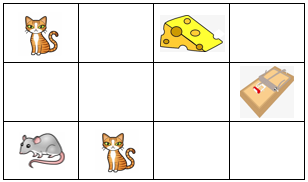
\includegraphics[width=5cm, height=5cm]{pic-toro/exam/cat.png}
    \end{center}
    \begin{enumerate}
        \item ขึ้น ขวา ขวา ขึ้น
        \item ขึ้น ขวา ขวา ขวา
        \item ขึ้น ขึ้น ขวา ขวา
        \item ขึ้น ลง ขวา ขวา
    \end{enumerate}
    \item จากรูปจงเขียนลูกศรนำทางให้เด็กชายไปเอากุญแจเพื่อมาเปิดกล่องสมบัติ
    \begin{center}
        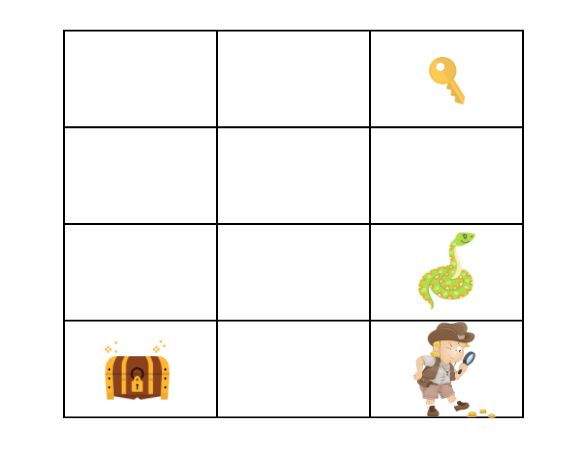
\includegraphics[width=5cm, height=5cm]{pic-toro/exam/treasure.png}
    \end{center}
    \item จากรูปจงเขียนลูกศรนำทางให้เด็กชายไปเอากุญแจเพื่อมาเปิดกล่องสมบัติ
    \begin{center}
        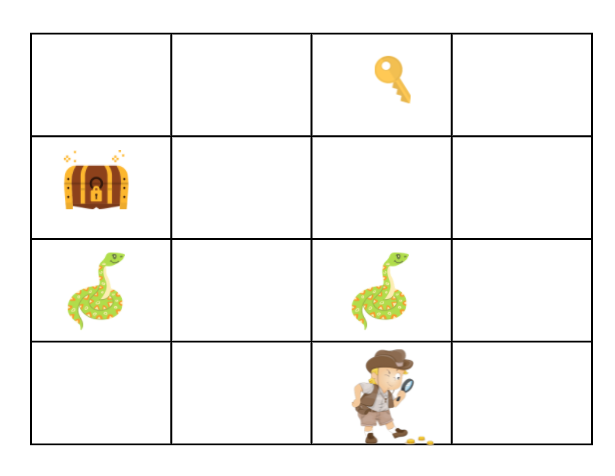
\includegraphics[width=5cm, height=5cm]{pic-toro/exam/treasure2.png}
    \end{center}
    \item นำทางคนป่ากลับถ้ำโดยใช้ลูกศร
    \begin{center}
        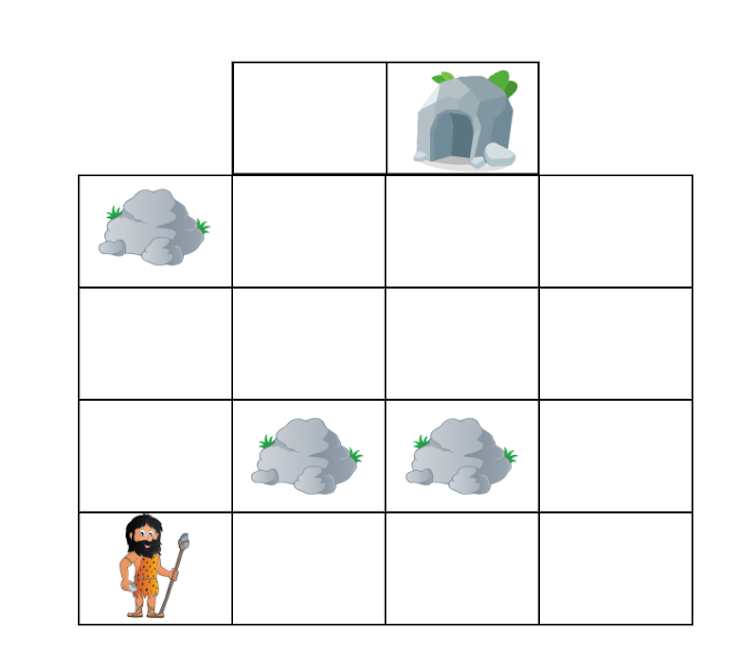
\includegraphics[width=5cm, height=5cm]{pic-toro/exam/cave.png}
    \end{center}
    \item นำทางหนูไปหาชีสโดยที่ไม่ต้องเจอแมว
    \begin{center}
        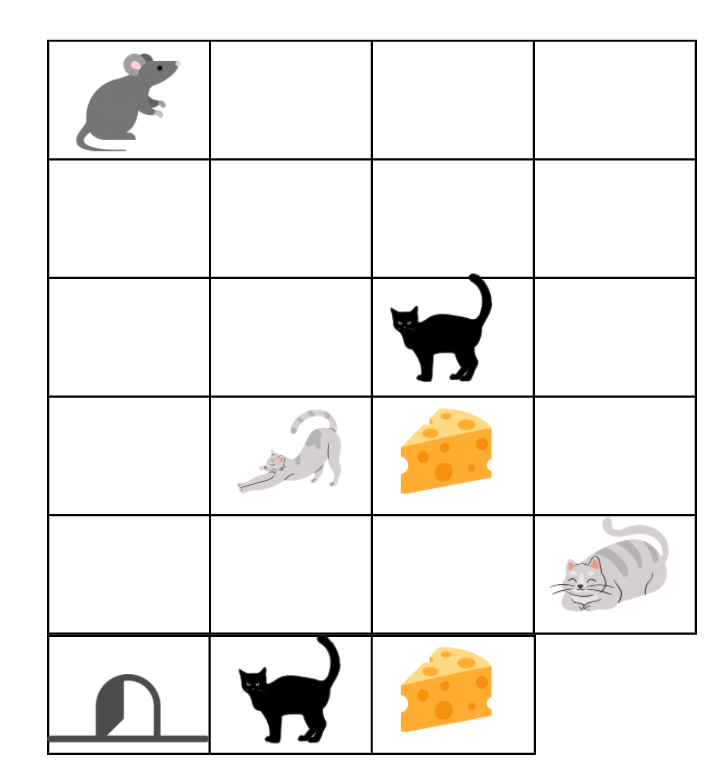
\includegraphics[width=5cm, height=5cm]{pic-toro/exam/cathard.png}
    \end{center}
\end{enumerate}

\section{ตัวอย่าง post-test}
\begin{enumerate}
    \item ข้อใดกล่าวถึงหลักการคิดเชิงคำนวณได้ถูกต้อง
    \begin{enumerate}
        \item เป็นการแก้ปัญหาแบบมีลำดับขั้นตอน
        \item เป็นทักษะที่นักพัฒนาซอฟต์แวร์ต้องมี
        \item เป็นการคิดเหมือนหุ่นยนต์
        \item ข้อ 1 และ ข้อ 2 ถูกต้อง
    \end{enumerate}
    \item จงเรียงลำดับการข้ามถนนบนทางม้าลายที่มีสัญญาณไฟจราจรคนข้ามถนนให้ถูกต้อง
    \begin{itemize}
        \item ไฟจราจรสีเขียว "ข้ามได้"
        \item สังเกตสัญญาณไฟจราจรคนข้ามถนน
        \item เดินข้ามถนนตรงทางม้าลาย
        \item กดปุ่มสัญญาณไฟจราจรคนข้ามถนน
        \item ไฟจราจรสีแดง "หยุดรอ"
    \end{itemize}
    \item กระบวนการแก้ปัญหาจะต้องเริ่มจากขั้นตอนใดเป็นขั้นตอนแรก
    \begin{enumerate}
        \item ดำเนินการแก้ไข
        \item วางแผนการแก้ปัญหา
        \item ตรวจสอบและปรับปรุง
        \item วิเคราะห์และกำหนดรายละเอียดของปัญหา
    \end{enumerate}
    \item ถ้านักเรียนต้องจัดกระเป๋าเพื่อไปเที่ยว ขั้นตอนใดเรียงลำดับได้เหมาะสมที่สุด
    \begin{enumerate}
        \item อาบน้ำ > แต่งตัว > สตาร์ทรถ > เติมน้ำมัน > จัดกระเป๋า
        \item สตาร์ทรถ > เติมน้ำมัน > อาบน้ำ > จัดกระเป๋า > แต่งตัว
        \item อาบน้ำ > แต่งตัว > จัดกระเป๋าอาบน้ำ > สตาร์ทรถ > เติมน้ำมัน
        \item จัดกระเป๋า > อาบน้ำ > แต่งตัว > สตาร์ทรถ > เติมน้ำมัน
    \end{enumerate}
    \item ข้อใดเรียงลำดับการใช้งานคอมพิวเตอร์ได้อย่างเหมาะสมที่สุด
    \begin{enumerate}
        \item เสียบปลั๊ก > กดปุ่มเปิดเครื่อง > กดปุ่มเปิดหน้าจอ > ใช้งาน > กด Shutdown > ปิดหน้าจอ > ถอดปลั๊ก
        \item เสียบปลั๊ก > กดปุ่มเปิดหน้าจอ > ใช้งาน > กด Shutdown > ปิดหน้าจอ > ถอดปลั๊ก
        \item เสียบปลั๊ก > กดปุ่มเปิดเครื่อง > กดปุ่มเปิดหน้าจอ > ใช้งาน > ปิดหน้าจอ > ถอดปลั๊ก
        \item เสียบปลั๊ก > กดปุ่มเปิดหน้าจอ > กดปุ่มเปิดเครื่อง > ใช้งาน > ถอดปลั๊ก > ปิดหน้าจอ
    \end{enumerate}
    \item ช่วยผึ้งหนีหมีและเก็บดอกไม้ไปยังรังผึ้ง
    \begin{center}
        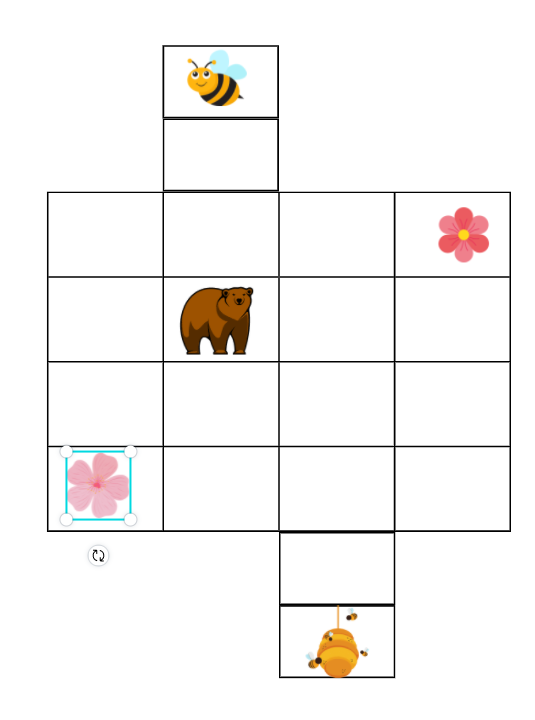
\includegraphics[width=5cm, height=5cm]{pic-toro/exam/bee.png}
    \end{center}
    \item จงลากดินสอไปหาเลข 1 2 3 ตามลำดับแล้วไปยังเส้นชัย
    \begin{center}
        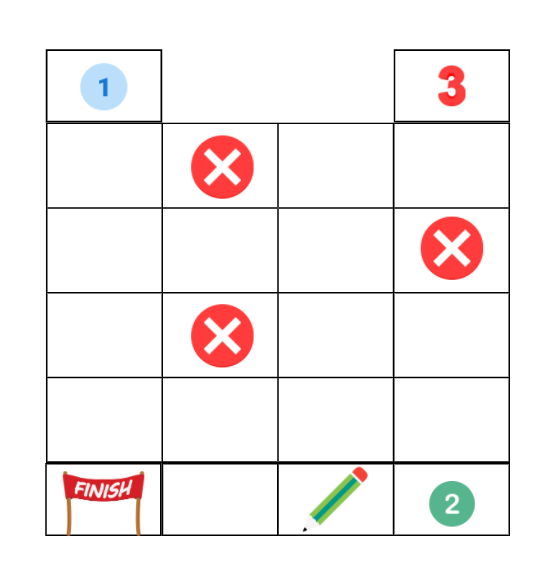
\includegraphics[width=5cm, height=5cm]{pic-toro/exam/pen.png}
    \end{center}
    \item จงรดน้ำต้นไม้ให้ครบทุกต้น
    \begin{center}
        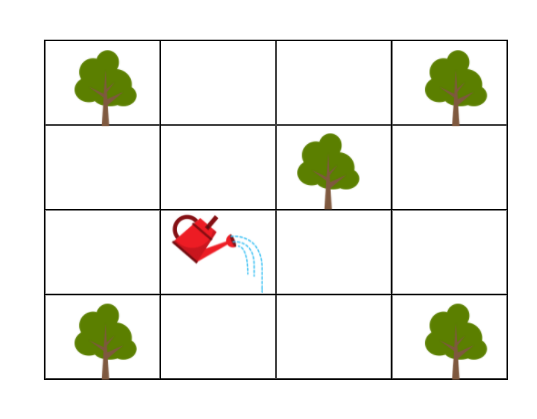
\includegraphics[width=5cm, height=5cm]{pic-toro/exam/treeeasy.png}
    \end{center}
    \item หาวิธีรดน้ำต้นไม้ให้ครบทุกต้นโดยใช้จำนวนครั้งในการเดินน้อยที่สุด
    \begin{center}
        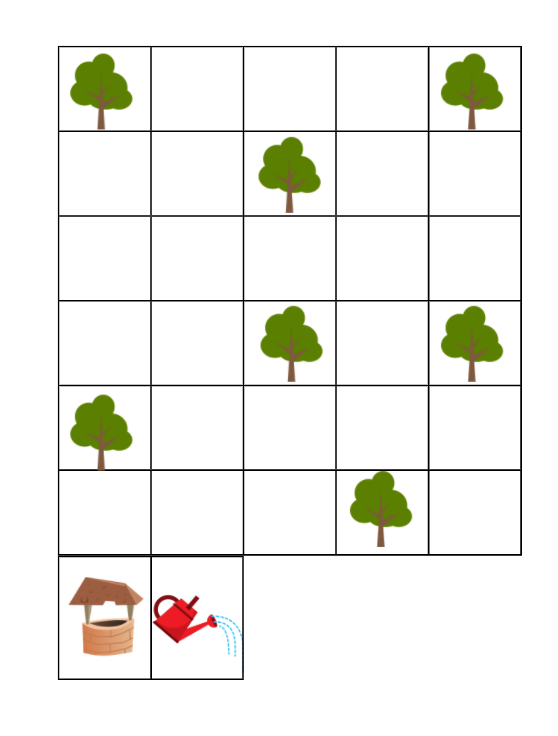
\includegraphics[width=5cm, height=5cm]{pic-toro/exam/treemed.png}
    \end{center}
    \item รดน้ำต้นไม้ให้ครบทุกต้นโดยที่บัวรดน้ำ 1 อันรดน้ำต้นไม้ได้ 3 ครั้ง จากนั้นต้องกลับมาเติมใหม่
    \begin{center}
        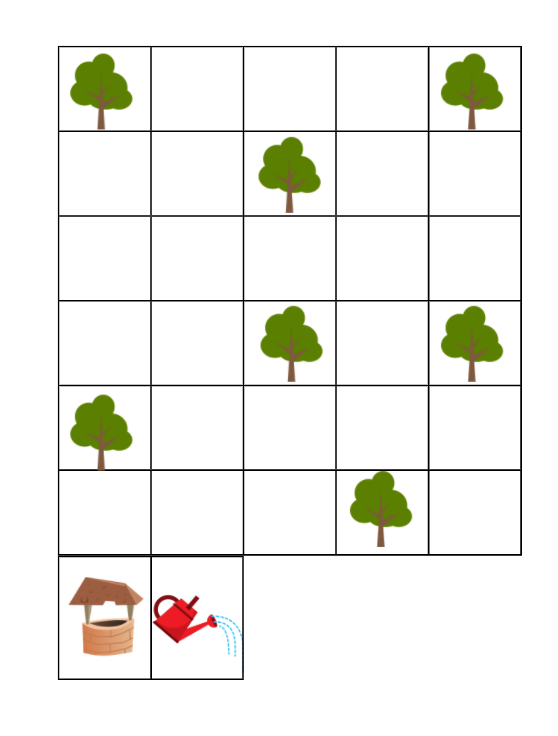
\includegraphics[width=5cm, height=5cm]{pic-toro/exam/treehard.png}
    \end{center} 
\end{enumerate}

\chapter{\ifcpe คู่มือการใช้งานระบบ\else Manual\fi}

เกมแอปพลิเคชันของโครงงานนี้ จะเป็นเกมแนวอาร์เคดที่สามารถเล่นได้ทุกเพศทุกวัย 
เป็นเกมที่เล่นโดยใช้ทักษะการคิดเชิงคำนวณ เพื่อเล่นให้ผ่านในแต่ละด่าน เก็บคะแนนที่จะได้เป็นดาว แล้วปลดล็อกด่านต่อไปเรื่อยๆ 
โดยภายในเกมจะมีแผนที่อยู่ด้วยกันทั้งหมด 3 แผนที่ แต่ละแผนที่จะมีสภาพแวดล้อมที่แตกต่างกัน และมีด่านอยู่ภายในทั้งหมด 10 
ด่าน แต่ละด่านก็จะมีความยากง่ายแตกต่างกัน โดยจะมีความซับซ้อนและมีเงื่อนไขใหม่ๆ
เพิ่มเข้ามา เพื่อให้ผู้เล่นได้ใช้และพัฒนาทักษะการคิดเชิงคำนวณมากขึ้น

\section{การใช้งานพื้นฐาน}
\begin{enumerate}
    \item หน้าเมนูหลัก กดปุ่ม Start เพื่อไปยังหน้าหน้าเลือกแผนที่ที่ได้ทำการปลดล็อกแล้ว หากต้องการจะกลับมายังหน้าเมนูหลัก ให้กดปุ่ม Home
    \item หน้าเลือกแผนที่ ให้ทำการเลือกแผนที่ที่ต้องการเล่น จากทั้งหมด 3 แผนที่ โดยเริ่มต้นจะปลดล็อกเพียงแผนที่แรกเท่านั้น ผู้เล่นต้องทำการเล่นเก็บดาวเพื่อมาปลดล็อกแผนที่ถัดๆ ไป ดาวที่ผู้เล่นได้รับจะแสดงอยู่มุมขวาบนของหน้าจอ \CI{ดังรูปที่}{?}\ref{mapselection}
    \item หน้าเลือกด่านจะประกอบไปด้วยด่านทั้งหมด 10 ด่าน ในแต่ละด่านจะมีดาวให้เก็บ 3 ดาว ระบบจะวัดผลจากคะแนนที่ได้ในด่านนั้นให้เป็นดาว โดยต้องผ่านอย่างน้อย 1 ดาวจึงจะไปยังด่านต่อไปได้
    \item เมื่อผ่านด่านแล้ว จะมีปุ่มให้เลือกกดไปยังด่านถัดไป หากไม่ผ่านด่าน ต้องทำการเล่นอีกครั้งจนกว่าจะได้อย่างน้อย 1 ดาว
\end{enumerate}

\section{วิธีการเล่น}
\begin{enumerate}
    \item เมื่อเริ่มเกม ตัวละครจะอยู่ห่างจากจุดหมายระยะหนึ่ง ให้นำพาตัวละครไปยังจุดหมายโดยใช้หลักการคิดเชิงคำนวณในวิเคราะห์เส้นทาง 
    
\end{enumerate}

\section{สัญลักษณ์ปุ่มต่างๆภายในเกม}



%% Display glossary (optional) -- need glossary option.
\ifglossary\glossarypage\fi

%% Display index (optional) -- need idx option.
\ifindex\indexpage\fi

\begin{biosketch}
\begin{center}
  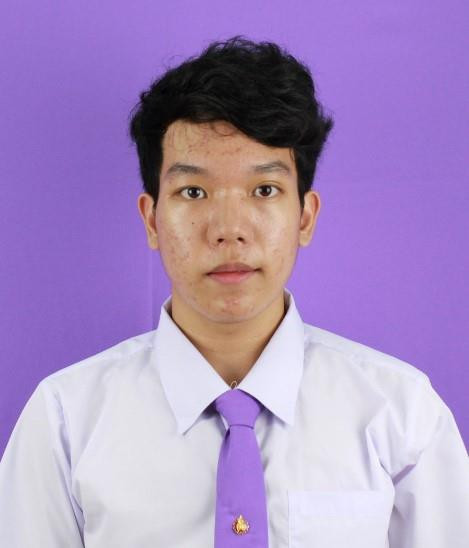
\includegraphics[width=1.5in]{pic-toro/me.jpg}
\end{center}
นาย กรวิชญ์ บัวคำปัน เกิดเมื่อวันที่ 27 กันยายน 2543 ณ จังหวัดเชียงใหม่ สำเร็จการศึกษาระดับมัธยมจากโรงเรียนวิชัยวิทยาอิงลิชโปรแกรม โดยเข้าศึกษาต่อที่คณะวิศวกรรมศาสตร์ สาขาคอมพิวเตอร์ มหาวิทยาลัยเชียงใหม่ ปีการศึกษา 2561
โดยมีความสนใจในด้านอุตสาหกรรมเกม และซอฟแวร์ต่างๆ ในระหว่างการศึกษาผู้พัฒนาได้เข้าร่วมโครงการต่างๆ ดังนี้ เข้าร่วมโครงการ Social Driver สำหรับ Start-Up ชิงเงินรางวัลเพื่อนำไปต่อยอดในธุรกิจ Start-Up โดยได้ผ่านเข้าสู่รอบชิงชนะเลิศของโครงการ
และได้เข้าร่วมการแข่งขันพัฒนาโปรแกรมคอมพิวเตอร์แห่งประเทศไทย หรือ National Software Contest - NSC ครั้งที่ 23 โดยผ่านการคัดเลือกเข้ารอบสุดท้ายและได้รับรางวัลชมเชย รวมถึงทางผู้พัฒนาเองมีประสบในด้านการจัดการศึกษาเนื่องด้วยระหว่างการศึกษา
ทางผู้พัฒนาเองได้มีโอกาศในการจัดการอบรม Coding และ STEM ให้กับครูวิทยาศาสตร์ และได้เป็นผู้พัฒนาสื่อเกมในการเรียนการสอนวิชาคณิตศาสตร์โรงเรียนดาราวิทยาลัยเพื่อให้ครูนำไปสอนนักเรียน
\newline
\begin{center}
  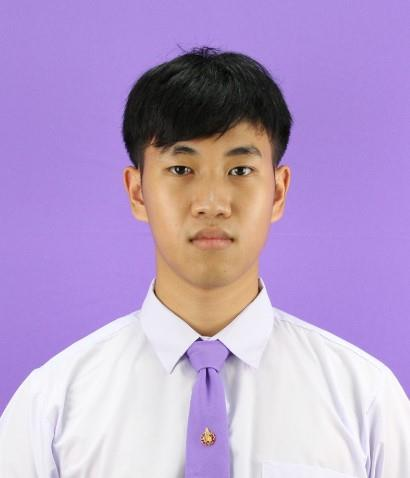
\includegraphics[width=1.5in]{pic/ToonImg.jpg}  
\end{center}
นาย กิตติพงษ์ ไมล์หรือ เกิดเมื่อวันที่ 3 ธันวาคม 2542 ณ จังหวัดเชียงราย สำเร็จการศึกษาระดับมัธยมจากโรงเรียนสามัคคีวิทยาคม เข้าศึกษาที่ภาควิชาวิศวกรรมคอมพิวเตอร์ มหาวิทยาลัยเชียงใหม่ เมื่อ สิงหาคม 2561 โดยมีความสนใจเป็นพิเศษในด้านการพัฒนาฮาร์ดแวร์ ระบบ IoT ออกแบบแอปพลิเคชัน และสนใจด้านธุรกิจต่าง ๆ\newline 
ระหว่างศึกษาได้เจ้าร่วมกิจกรรมต่าง ๆ ในด้านวิชาการ  โดยได้เข้าร่วมกิจกรรมการแข่งขัน Startup โครงการ Social Driver ที่จัดขึ้นโดย อุทยานวิทยาศาสตร์และเทคโนโลยี มหาวิทยาลัยเชียงใหม่ (STeP) โดยได้ผ่านเข้าสู่รอบชิงชนะเลิศ และได้เป็นส่วนหนึ่งในการพัฒนาโปรแกรม ที่นำไปเข้าร่วมการแข่งขันพัฒนาโปรแกรมคอมพิวเตอร์แห่งประเทศไทย 
หรือ National Software Contest - NSC ครั้งที่ 23 โดยผ่านการคัดเลือกเข้าสู่รอบคัดเลือกระดับภาคและได้รับรางวัลชมเชย
the \texttt{biosketch} environment.

\end{biosketch}
\fi % \ifproject
\end{document}
